% Long-form version. The 5-page submission version is paper/talk_like_a_graph.tex.
% Everything here is either (a) restored material cut from that version purely for
% length, or (b) analysis that was never in the paper at all -- see paper/LONG.md.
\documentclass[11pt]{article}

% "preprint" = numbered pages, authors visible, no review line numbers.
% Switch to [final] for a camera-ready, or [review] for double-blind.
\usepackage[preprint]{acl}

\usepackage{times}
\usepackage{latexsym}
\usepackage[T1]{fontenc}
\usepackage[utf8]{inputenc}
\usepackage{microtype}
\usepackage{graphicx}
\usepackage{booktabs}
\usepackage{multirow}
\usepackage{float}

\title{Primers and Shortcuts: Testing Structural Preambles for LLM Graph Reasoning at Scale}

\author{
  Gal Barak \\
  \footnotesize\texttt{github.com/GalBrk} \\\And
  Nitzan Zacharia \\
  \footnotesize\texttt{github.com/NitzanZacharia} \\\And
  Inbal Moryles \\
  \footnotesize\texttt{github.com/iinbal} \\
}

\begin{document}
\maketitle

\begin{abstract}
Prepending a short \emph{primer} of factual sentences about each node's
local structure --- degree, clustering coefficient, a random-walk
structural encoding, or connected-component membership --- before a
graph's standard text encoding is an intuitively appealing way to ease
graph-reasoning prompts for a large language model. Any apparent gain is
illusory, however, if a solver can recover the answer directly from the
primer text without ever consulting the graph, and it is confounded if the
primer merely lengthens the prompt. We introduce a graph-blind shortcut
solver as a content-only lower bound and a length-matched filler control as
a length-only upper bound. Evaluated at $n=40$ on \texttt{qwen3-1.7b} and
\texttt{qwen3-4b}, with and without chain-of-thought --- $67{,}200$
generations across six GraphQA tasks, seven primer conditions and four edge
densities --- we find that no primer effect replicates across model scale.
Several cells beat both \texttt{none} and \texttt{filler} significantly in
one model size, but none does so in both. The largest consistent content
effect --- the \texttt{degree} primer on \texttt{node\_degree}, which states
the answer verbatim --- reverses sign between 1.7B ($+7.5$ points) and 4B
($-6.5$). Nor is the filler inert: it costs the thinking arm up to $14.1$
points on dense graphs and harms both sizes on \texttt{edge\_existence}.
The largest apparent gains fall on tasks whose answer is effectively
constant, where content-free text moves accuracy as much as a structural
primer does. Chain-of-thought on an identical checkpoint is worth $+29.2$
points pooled, an order of magnitude more than any primer effect measured.
One cell survives every control: \texttt{clustering} on
\texttt{node\_degree} for \texttt{qwen3-1.7b}, $+3.8$ points, replicated at
$+4.3$ on an independent sample ($p=0.0006$).
\end{abstract}

\section{Introduction}
\label{sec:introduction}

\citet{fatemi2023talklikeagraph} demonstrate that a large language model's
accuracy on graph-reasoning questions depends substantially on how the
graph is encoded as text, independent of the model's underlying reasoning
ability. Their study varies the encoding function itself --- adjacency
lists, incident lists, and a family of ``themed'' encodings that rename
nodes as people, places, or characters --- while holding the question and
the underlying graph fixed.

This work poses a complementary question: rather than altering how edges
are described, does prepending a short \emph{primer} of derived,
node-level facts before the graph encoding help a model answer questions
about that graph? A primer lies outside the encoding vocabulary studied by
\citet{fatemi2023talklikeagraph}: it is additional, redundant information
computed from the graph and expressed in plain sentences, a term this
project introduces for it. The appeal is obvious --- if a model miscounts a
node's neighbours in a dense incident list, telling it the degree outright
ought to help --- and so is the risk.

Two confounds make such an effect hard to read, and both are easy to
overlook. If a primer condition helps only because it lets the model read
the answer directly from the primer text rather than reason over the graph,
that is not evidence of increased graph reasoning; it is evidence that the
primer leaked the answer. And if a primer helps or hurts only because it
lengthens the prompt, that is not evidence about its \emph{content} either.
\citet{liu2024lostinthemiddle} and the needle-in-a-haystack protocol of
\citet{kamradt2023needle} show that context position and length alone move
retrieval accuracy, whatever the added text says. A primer study that
compares each condition only against a no-primer baseline measures the sum
of three things --- content, leakage and length --- and reports it as one.

This paper makes two contributions aimed squarely at separating them.
First, a single, deterministic primer renderer that produces seven
conditions (Section~\ref{sec:primers}) differing only in content, so that
differences between conditions are interpretable as content effects rather
than formatting artifacts. Among those seven is a length-matched,
information-free \texttt{filler} condition that bounds how much of any
effect is attributable to prompt length alone. Second, a \emph{shortcut
solver} (Section~\ref{sec:shortcuts}) that answers each GraphQA task from
rendered primer text alone, with no access to the graph, yielding a
principled lower bound that any genuine primer benefit must exceed. We
evaluate both within a density sweep of GraphQA tasks on two model sizes,
\texttt{qwen3-1.7b} and \texttt{qwen3-4b}, each with and without
chain-of-thought (Section~\ref{sec:setup}).

The result is largely negative, and the controls are what make it
informative rather than merely disappointing. Of the effects that do reach
significance, the reliable ones are answer retrieval and the large ones are
length. What headroom remained for anything else was mostly consumed by the
decoding mode.

\section{Related Work}
\label{sec:related-work}

\citet{fatemi2023talklikeagraph} introduce GraphQA, a benchmark of graph
reasoning tasks --- node degree, node count, edge count, edge existence,
connected nodes, cycle check, and disconnected nodes --- paired with a
family of graph-to-text encoding functions. They show that encoding choice,
task, and the underlying graph generator all materially affect LLM
accuracy. This project adopts their task definitions. Their finding that
the generator matters is what motivates fixing graph size and edge density
explicitly in our own design (Section~\ref{sec:setup}), rather than
sampling graph structure incidentally.

We verified this directly before finalizing the design, and the result is
worth recording because it closed off an experiment we had intended to run.
We swept the generator itself: Erd\H{o}s--R\'enyi
\citep{erdosrenyi1959random}, Barab\'asi--Albert, random regular,
Watts--Strogatz, and stochastic block models, at matched node and edge
counts. The majority-class baseline moved from $0.15$ to $1.0$, a swing six
times larger than any primer effect measured anywhere in this project.
Random-regular graphs were degenerate outright: every instance shares a
single gold answer. A generator-family sweep was accordingly withdrawn. It
confounds structural family with task difficulty rather than isolating a
structural effect, which is the very failure the \texttt{filler} control
exists to prevent.

A broader literature probes LLM graph reasoning more generally.
\citet{wang2023nlgraph} evaluate eight graph tasks of increasing
complexity and report that LLMs are brittle to spurious correlations in
graph and problem structure, the same concern that motivates our shortcut
solver (Section~\ref{sec:shortcuts}), applied here to the primer channel
rather than to the graph encoding. \citet{guo2023gpt4graph} instead encode
graphs through standard graph description languages (GML, GraphML) and
find that LLMs struggle to exploit that structure directly, and
\citet{jin2024largelanguagemodelsongraphs} survey the broader space of
LLM-graph integration methods within which this project sits.
\citet{dziri2023faithandfate} argue that transformers solve compositional
tasks --- multi-digit multiplication, dynamic programming --- by
linearized subgraph matching rather than systematic multi-step reasoning.
That finding raises the question a primer's apparent benefit also raises:
is an observed gain evidence of reasoning, or of a shorter pattern to match
against? \citet{geirhos2020shortcut} frame the concern generally as
\emph{shortcut learning}, a decision rule that performs well on the
benchmark it was measured against without solving the intended problem. Our
shortcut solver operationalizes that concern for the primer channel, rather
than for the model as a whole.

The RWSE primer condition (Section~\ref{sec:primers}) adapts the
random-walk structural encoding of \citet{dwivedi2022graph}, originally
developed for graph transformers rather than for text prompts; we render
its return probabilities as natural-language sentences rather than feeding
them to an attention mechanism. The chain-of-thought variant of our sweep
follows \citet{wei2022chainofthought}, who show that eliciting
step-by-step reasoning changes what a model can accomplish on structured
tasks, consistent with the reasoning-mode effect we observe in
Section~\ref{sec:results-cot}, which dwarfs every primer effect measured.
Our significance-testing methodology (Section~\ref{sec:significance})
follows the general recommendation of \citet{dror2018hitchhikers} to test
the actual dependence structure of paired evaluation data rather than treat
each item as independent.

\section{Method}
\label{sec:method}

\subsection{Primers}
\label{sec:primers}

A primer is a short preamble of factual sentences that details a graph's
local or global structure, prepended to the standard text encoding and the
task question. To ensure that observed differences reflect genuine content
effects rather than formatting artifacts, a single renderer produces every
condition: all node-level facts consequently share identical sentence
framing (e.g., ``Node $N$ has\dots''), and floating-point values are rounded
and formatted identically across conditions. We evaluate seven distinct
conditions:
\begin{itemize}
    \item \textbf{None}: The baseline graph text encoding without a
    primer.
    \item \textbf{Components}: A single graph-level sentence stating the
    number of connected components.
    \item \textbf{Degree}: The exact degree reported for each node.
    \item \textbf{Clustering}: The clustering coefficient computed for
    each node.
    \item \textbf{RWSE}: The random-walk structural encoding
    \citep{dwivedi2022graph} return probabilities for each node.
    \item \textbf{All}: The degree, clustering, and RWSE statistics
    combined for every node.
    \item \textbf{Filler}: A content-free control matched in length to the
    factual primers, e.g.\ ``Node $N$ is simply present within the graph
    $G$.'' It isolates primer content from the confound of prompt length.
\end{itemize}

\begin{table}[t]
\centering
\footnotesize
\setlength{\tabcolsep}{4pt}
\begin{tabular}{lrl}
\toprule
Condition & Chars & Rendered form (node 0) \\
\midrule
\texttt{none}       &    0 & --- \\
\texttt{components} &   39 & \emph{(one sentence, graph-level)} \\
\texttt{degree}     &  897 & ``has degree 5.'' \\
\texttt{clustering} & 1631 & ``has clustering coefficient 0.20.'' \\
\texttt{filler}     & 1831 & ``is simply present within $G$.'' \\
\texttt{rwse}       & 2951 & ``has return probability 0.27 after \\
                    &      & ~~2 steps and 0.04 after 3 steps.'' \\
\texttt{all}        & 4697 & \emph{(the three above, conjoined)} \\
\bottomrule
\end{tabular}
\caption{The seven conditions at $n{=}40$: median rendered primer length in
characters over $400$ prompts, and the sentence each emits for a single
node. Every node-level condition emits exactly one sentence per node, so
the conditions differ in what the sentence asserts and in nothing else.
\texttt{components} emits one sentence for the whole graph, which is why it
is two orders of magnitude shorter than the rest --- the one condition
whose effect cannot be confounded with length.}
\label{tab:lengths}
\end{table}

Table~\ref{tab:lengths} gives the rendered length of each condition at the
graph size used throughout. Two features of it matter for interpretation.
\texttt{components} is $39$ characters against \texttt{all}'s $4{,}697$, so
it is effectively a length-free intervention and any effect it shows is
content. And \texttt{filler}, at $1{,}831$ characters, falls between
\texttt{clustering} ($1{,}631$) and \texttt{rwse} ($2{,}951$): it brackets
the informative primers rather than matching any single one exactly, so it
bounds the length term rather than cancelling it.

\subsection{Shortcut solvers}
\label{sec:shortcuts}

For a primer condition's measured accuracy on a task to constitute
evidence of graph reasoning, it must exceed what is recoverable from the
primer text alone. We construct a shortcut solver that takes only rendered
primer text as input --- never the graph object, and never the
full-precision statistics the primer rounds away --- and answers each
GraphQA task directly. It combines four kinds of rule: sixteen exact ones,
such as deriving edge count algebraically from a \texttt{degree} primer,
since the stated degrees sum to $2m$; one heuristic; eight fitted rules,
whose fitting and scoring graph sets are kept structurally disjoint so that
accuracy is not inflated by evaluating on the fitting data; and an exact
enumeration bound for small graphs.

The solver is \emph{structurally} incapable of observing the graph. It
takes rendered text as its only argument, so there is no graph to pass and
no discipline to violate. Its accuracy on a given (primer condition, task)
cell is therefore a model-independent bound, and model results on that cell
should be read against this \emph{shortcut ceiling} rather than against
zero. Where a primer fully determines the answer --- a ceiling of $1.0$ ---
model accuracy is uninformative about graph reasoning, however high it may
be.

\begin{table}[t]
\centering
\footnotesize
\setlength{\tabcolsep}{3.2pt}
\resizebox{\columnwidth}{!}{%
\begin{tabular}{lrrrrrrr}
\toprule
Task & none & comp. & clust. & rwse & degree & filler & all \\
\midrule
\texttt{node\_count}      & .064 & .076 & \textbf{1.00} & \textbf{1.00} & \textbf{1.00} & \textbf{1.00} & \textbf{1.00} \\
\texttt{edge\_count}      & .018 & .018 & .148 & .018 & \textbf{1.00} & .018 & \textbf{1.00} \\
\texttt{node\_degree}     & .082 & .082 & .082 & .616 & \textbf{1.00} & .082 & \textbf{1.00} \\
\texttt{connected\_nodes} & .082 & .082 & .082 & .082 & .208 & .082 & .352 \\
\texttt{edge\_existence}  & .498 & .498 & .720 & .642 & .794 & .498 & .794 \\
\texttt{cycle\_check}     & .832 & \textbf{1.00} & .832 & .832 & .946 & .832 & .946 \\
\bottomrule
\end{tabular}}
\caption{Shortcut ceilings: accuracy of a solver that reads only the
rendered primer and never the graph, over $500$ graphs from the GraphQA
generator. \textbf{Bold} marks cells the primer fully determines, on which
no model result can be evidence of graph reasoning. Four of six tasks are
decided this way for at least one primer. Note that a $1.00$ here is what a
Python program scores, not what a model scores: on \texttt{node\_count} the
ceiling is $1.00$ and \citet{fatemi2023talklikeagraph} report $18.8\%$ for
PaLM 2 on the encoding GraphQA ships. A decided cell still answers a
question, but a narrower one --- whether the model uses a fact it was
handed, not whether it reasoned about the graph.}
\label{tab:shortcut}
\end{table}

Table~\ref{tab:shortcut} gives the resulting ceilings. They sort the sweep
rather than pruning it. Three of the sixteen exact rules \emph{reconstruct}
rather than compare: a stated degree sequence constrains which graphs are
possible, often to exactly one, so a primer that states no adjacency at all
can still give away whole neighbour lists. That is why
\texttt{connected\_nodes} under \texttt{all} is a $35.2\%$ cell rather than
the $8.2\%$ one it first appears to be.

\subsection{Prompt assembly}
\label{sec:prompts}

Each prompt concatenates the primer, the graph's text encoding, and the
task question. Prompts are rebuilt from a canonicalized, parsed
representation of each graph rather than reused verbatim from the source
dataset, so that node and edge ordering is reproducible and independent of
the order in which the original question happened to list them. We use the
\texttt{incident} encoding throughout, which emits one line per node; the
published dataset ships the \texttt{adjacency} encoding in its
\texttt{question} field, which is why prompts are regenerated rather than
reused.

\subsection{Significance testing}
\label{sec:significance}

Every comparison reported here is paired: a primer condition is compared
against \texttt{none} on the same graph, with the same question and gold
answer, and pairs in which either arm reached the output-token cap are
dropped from that comparison rather than scored as incorrect
(Section~\ref{sec:results-sensitivity} reports what the opposite convention
would do). Because a graph contributes exactly one pair to a given (task,
condition) comparison, the pairs entering a single test are independent and
no clustering correction is required; we do not pool across tasks, where
they would not be \citep{dror2018hitchhikers}.

The primary test is the exact McNemar test \citep{mcnemar1947note},
Benjamini--Hochberg corrected across the six primer conditions within a
task \citep{benjaminihochberg1995controlling} --- $q=0.05$, six hypotheses
per family, rather than one family of $144$: a primer's effect on
\texttt{node\_count} and its effect on \texttt{cycle\_check} are not
alternative answers to one question. For every comparison we additionally
report two resampling statistics (Appendix~\ref{sec:appendix-ci}). The
first is a paired permutation test, sign-flipping each pair's observed
difference over $20{,}000$ resamples with the add-one correction of North
et al. The second is a paired bootstrap $95\%$ confidence interval on the
effect size, resampling whole pairs $20{,}000$ times. The permutation and
McNemar $p$-values agree to within a few thousandths on every cell, so the
interval, not the second $p$-value, is what the extra computation buys.

\subsection{Answer extraction and measurement validity}
\label{sec:extraction}

Turning free model text into a scored answer is the quiet source of
measurement error in a study of this shape, and the error is not symmetric
across conditions. Chain-of-thought responses are longer and messier than
zero-shot ones, so a naive extractor makes the thinking arm look worse than
it is --- and that is one of the comparisons we want to draw. Extraction is
therefore written per task and tested against the shapes models actually
emit, rather than being a single regular expression.

One failure is worth reporting in full, because it silently produced a
headline-sized effect that does not exist. Our boolean extractor took the
last yes/no token in the response. On \texttt{cycle\_check},
\texttt{qwen3-4b} frequently answers correctly and then recites the
definition: \emph{``Yes, there is a cycle. A cycle is a path \dots with no
repeated edges or nodes.''} The trailing ``no'' became the extracted
answer. Correcting the extractor to ignore the phrase ``no repeated''
changed $225$ of \texttt{qwen3-4b}'s $5{,}568$ scored boolean rows, every
one of them from wrong to right, and every one on \texttt{cycle\_check};
no row moved in the other direction. Before the fix, \texttt{filler} scored
$0.140$ at $p{=}0.2$ and \texttt{none}, \texttt{all} and \texttt{rwse}
scored $0.86$, $0.64$ and $0.51$ at $p{=}0.5$, which reads as a dramatic
condition-dependent collapse. After it, every condition scores $0.97$ to
$1.00$ and nothing on that task is significant. All numbers in this paper
use the corrected extractor. We note this not as a curiosity but as a
pattern: an extraction bug that correlates with response style will
manifest as a condition effect, and there is nothing in the resulting
table that looks wrong.

\section{Experimental Setup}
\label{sec:setup}

\paragraph{Tasks.} We evaluate on six GraphQA tasks from
\citet{fatemi2023talklikeagraph}: node count, edge count, node degree,
connected nodes, edge existence, and cycle check.

\paragraph{Models.} We compare \texttt{qwen3-1.7b} and \texttt{qwen3-4b}
from the Qwen3 model family \citep{qwen2025qwen3}, each evaluated in a
non-thinking (greedy decoding, no chain-of-thought) and a thinking
(chain-of-thought-enabled; \citealp{wei2022chainofthought}) variant, for
four model arms in total. Both families are pinned explicitly rather than
left at their defaults, which are opposite: left alone, Qwen3 would reason
in a hidden channel even in the nominally non-thinking arm, collapsing the
two arms into one condition.

\paragraph{Sweep design.} All four arms are evaluated on one shared set of
prompts, so that every model receives byte-identical inputs. Graphs are
Erd\H{o}s--R\'enyi \citep{erdosrenyi1959random} with a fixed node count of
40 and edge density swept over four levels ($p \in \{0.10, 0.20, 0.35,
0.50\}$). Every combination of the seven primer conditions
(Section~\ref{sec:primers}) and six tasks is evaluated on 100 graphs per
(density, task) cell, yielding 16{,}800 prompts per model arm and
$67{,}200$ generations in total. Generation is greedy, with a raised output
budget (up to 8192 tokens), since at the densest level tasks such as edge
count require enumerating several hundred edges in the answer.

\paragraph{Auxiliary sweeps.} Two comparisons need more power or a wider
density range than the main sweep provides, and use dedicated prompt sets
built by the same renderer. The first fixes \texttt{node\_degree} and
$400$ graphs per density level over the same four densities, for the
\texttt{clustering} comparison of Section~\ref{sec:results-headline}, and
was run twice on independently drawn graph samples. The second extends the
density range to $p \in \{0.10, \dots, 0.85\}$ on \texttt{node\_degree} for
the length and chain-of-thought comparisons of
Sections~\ref{sec:results-length} and~\ref{sec:results-cot}, where the main
sweep's ceiling at $p \le 0.50$ leaves too little dynamic range to measure
either. Both are identified explicitly wherever their numbers appear.

\paragraph{Metrics.} We use exact match for integer- and boolean-valued
tasks and set-F1 for connected nodes. Every result is reported against
both the \texttt{none} baseline and the shortcut ceiling for the
corresponding (primer condition, task) cell (Table~\ref{tab:shortcut}).
Generations that reach the output-token cap are excluded from scoring
rather than scored as incorrect, and are reported separately as a per-cell
drop count.

Note that we report \texttt{connected\_nodes} on exact match in the main
table even though F1 is its primary metric. Its F1 sits at $96$--$100\%$
for every condition in every arm, which conceals differences that exact
match resolves; and a McNemar test on F1 binarized as ``$>0$'' is
degenerate, since a partial-credit metric is almost never exactly zero, so
it reports $0$ to $1$ discordant pairs everywhere and would be misread as
``no effect''. The F1 figures are in Appendix~\ref{sec:appendix-density}.

\paragraph{Reproducibility.} All generation is greedy (no sampling), so a
run is deterministic given a checkpoint and a prompt file; the prompt files
are written to disk before any generation and shared byte-identically
across arms. Thinking and non-thinking arms are the same checkpoints with
the model's native reasoning channel pinned on or off, rather than a
prompt-level chain-of-thought instruction, so the two arms differ in
decoding mode alone. Code, prompt sets and raw generations are released
with the paper.

\paragraph{Known validity caveats.} At this graph size and density range,
several cells are known in advance to be shortcut-dominated rather than
genuine tests of graph reasoning: any primer with one sentence per node
allows node count to be recovered by counting sentences; cycle check's
gold answer is ``yes'' for nearly every graph past the sparsest density
level; and the \texttt{degree} primer states the node-degree answer
verbatim. The one cell already established as free of this contamination
at this graph size is node degree under \texttt{\{none, components,
clustering, filler\}}. We report and interpret results with this caveat in
mind rather than omitting the contaminated cells, since a null or negative
result on an uncontaminated cell remains informative in its own right.

\begin{table}[t]
\centering
\footnotesize
\setlength{\tabcolsep}{4pt}
\resizebox{\columnwidth}{!}{%
\begin{tabular}{llrrrr}
\toprule
Task & Modal answer & $0.10$ & $0.20$ & $0.35$ & $0.50$ \\
\midrule
\texttt{node\_count}      & ``40''    & 1.000 & 1.000 & 1.000 & 1.000 \\
\texttt{cycle\_check}     & ``Yes''   & 1.000 & 1.000 & 1.000 & 1.000 \\
\texttt{edge\_existence}  & ``No''    & 0.900 & 0.820 & 0.690 & 0.520 \\
\texttt{node\_degree}     & integer   & 0.210 & 0.170 & 0.170 & 0.180 \\
\texttt{edge\_count}      & integer   & 0.083 & 0.065 & 0.046 & 0.056 \\
\texttt{connected\_nodes} & node set  & 0.019 & 0.010 & 0.010 & 0.010 \\
\bottomrule
\end{tabular}}
\caption{Blind baselines: accuracy of always returning the modal gold
answer, by density. This is the floor a model must clear before any primer
effect on that task means anything, and it is the reason
\texttt{node\_count} and \texttt{cycle\_check} carry no information at
$n{=}40$ --- their gold answer is constant, so a model can be perfect
without reading the graph. Only \texttt{node\_degree},
\texttt{edge\_count} and \texttt{connected\_nodes} have real headroom at
every density.}
\label{tab:blind}
\end{table}

Table~\ref{tab:blind} makes the last caveat quantitative, and it is
important enough to state plainly: at $n{=}40$ the constant answer ``40''
scores $100\%$ on \texttt{node\_count} and the constant answer ``Yes''
scores $100\%$ on \texttt{cycle\_check}. Neither task measures graph
reasoning in this design. We report them because they turn out to measure
something else worth knowing (Section~\ref{sec:results-nodecount}), not
because they bear on the primer hypothesis.

\section{Results}
\label{sec:results}

All four model arms completed the full $n{=}40$ density sweep:
$16{,}800$ scored generations per arm, one per (task, primer, density,
graph) cell. Unless stated otherwise, every reported $\Delta$ is a
\emph{paired} difference against \texttt{none} on instances for which
neither arm reached the output-token cap, tested as described in
Section~\ref{sec:significance}. Complete per-density tables for every
(arm, task) pair are in Appendix~\ref{sec:appendix-density}, and effect
sizes with confidence intervals for all $144$ cells in
Appendix~\ref{sec:appendix-ci}.

\subsection{Truncation must be read before accuracy}
\label{sec:results-truncation}

\begin{table}[t]
\centering
\small
\begin{tabular}{lrrrr}
\toprule
& \multicolumn{2}{c}{1.7B} & \multicolumn{2}{c}{4B} \\
\cmidrule(lr){2-3}\cmidrule(lr){4-5}
Task & plain & think & plain & think \\
\midrule
\texttt{edge\_count}     & 22.4 & \textbf{81.0} & 0.6 & \textbf{62.3} \\
\texttt{cycle\_check}    &  6.1 &  6.5 & 1.0 &  1.9 \\
all others ($\max$)      &  0.8 &  2.5 & 0.1 &  3.5 \\
\midrule
Overall                  &  4.8 & 15.4 & 0.3 & 11.7 \\
\bottomrule
\end{tabular}
\caption{Truncation rate (\%~of generations reaching the 8192-token output
cap), by task and model arm.}
\label{tab:hitcap}
\end{table}

\begin{table}[t]
\centering
\footnotesize
\setlength{\tabcolsep}{3.4pt}
\begin{tabular}{lrrrrrrr}
\toprule
$p$ & none & comp. & clust. & rwse & degree & filler & all \\
\midrule
\multicolumn{8}{l}{\emph{\texttt{qwen3-1.7b} (plain)}} \\
0.10 & 31 & 20 & 10 & 10 & 10 & 15 & 26 \\
0.20 &  9 & 20 &  3 &  9 &  6 &  9 &  9 \\
0.35 & 50 & 33 & 26 & 21 &  2 & 40 & 33 \\
0.50 & 29 & 36 & 33 & 32 & 20 & 41 & 44 \\
\midrule
\multicolumn{8}{l}{\emph{\texttt{qwen3-4b-think}}} \\
0.10 &  60 & 27 & 20 & 31 & 64 & 40 & 50 \\
0.20 &  66 & 34 & 47 & 48 & 52 & 50 & 47 \\
0.35 &  92 & 65 & 51 & 91 & 59 & 77 & 63 \\
0.50 & \textbf{100} & 92 & 96 & 99 & 60 & 99 & 63 \\
\bottomrule
\end{tabular}
\caption{\texttt{edge\_count}: generations dropped to truncation, out of
$100$ per cell. The censoring is severe and \emph{condition-dependent},
which is worse than severe and uniform: at $p{=}0.5$, \texttt{none} loses
every row for \texttt{qwen3-4b-think} while \texttt{degree} loses $60$, so
the two arms of that comparison are scored on different graphs. The
\texttt{qwen3-1.7b-think} arm (not shown) has cells at $100\%$ from
$p{=}0.35$ upward.}
\label{tab:hitcap-detail}
\end{table}

Table~\ref{tab:hitcap} reports the fraction of generations that reach the
output-token cap. The rate is neither uniform across tasks nor across arms, and it is not
ignorable. On \texttt{edge\_count} the thinking arms truncate on
$62$--$81\%$ of instances, with individual (density, primer) cells at
$100\%$. Because truncated generations are dropped rather than scored as
incorrect, the survivors in those cells are a biased subset of the sparsest
graphs. The apparently high \texttt{none} accuracy there --- $86.3\%$ at
1.7B and $97.6\%$ at 4B, against $2\%$ in the corresponding untruncated
plain arms --- measures which graphs finished, not which were solved.

Table~\ref{tab:hitcap-detail} shows why this cannot be repaired by a
footnote. The drop rate varies by primer within a density, so the pairs
surviving a \texttt{degree}-vs-\texttt{none} comparison are not a random
subset of the pairs that entered it. We therefore report
\texttt{edge\_count} under chain-of-thought but decline to interpret it;
several of its comparisons rest on fewer than $60$ surviving pairs, and one
of the largest apparent effects in the entire sweep ($-61.5$ points for
\texttt{degree} on \texttt{qwen3-1.7b-think}) rests on $13$.

\subsection{The full density sweep}
\label{sec:results-main}

\begin{table*}[t]
\centering
\footnotesize
\setlength{\tabcolsep}{4.2pt}
\renewcommand{\arraystretch}{0.94}
\begin{tabular}{llrrrrrrr}
\toprule
Arm & Task & none & comp. & clust. & rwse & degree & filler & all \\
\midrule
\multirow{6}{*}{qwen3-1.7b}
 & connected\_nodes & 72.5 & $+0.8$ & $+1.2$ & $+1.0$ & $+3.5$ & $\mathbf{-6.2}$ & $+2.0$ \\
 & cycle\_check     & 99.7 & $-0.6$ & $+0.3$ & $\mathbf{-7.5}$ & $\mathbf{-12.6}$ & $+0.3$ & $-1.1$ \\
 & edge\_count      &  1.8 & $-1.4$ & $-0.4$ & $-0.8$ & $+4.0$ & $-0.4$ & $+2.4$ \\
 & edge\_existence  & 70.5 & $\mathbf{-8.2}$ & $+3.8$ & $+5.3$ & $+4.0$ & $\mathbf{-15.8}$ & $\mathbf{+11.5}$ \\
 & node\_count      & 31.5 & $\mathbf{+21.2}$ & $\mathbf{+67.2}$ & $+2.0$ & $\mathbf{+6.8}$ & $\mathbf{+39.8}$ & $\mathbf{+47.0}$ \\
 & node\_degree     & 60.5 & $+1.8$ & $+3.0$ & $+4.0$ & $\mathbf{+7.5}$ & $-0.5$ & $\mathbf{+10.2}$ \\
\midrule
\multirow{6}{*}{qwen3-1.7b-think}
 & connected\_nodes & 79.7 & $+2.8$ & $+1.5$ & $-0.3$ & $\mathbf{+7.4}$ & $+2.0$ & $\mathbf{+6.1}$ \\
 & cycle\_check     & 100.0 & $0.0$ & $0.0$ & $0.0$ & $-0.7$ & $0.0$ & $0.0$ \\
 & edge\_count$^{\dagger}$ & 86.3 & $+7.4$ & $-8.7$ & $-4.0$ & $\mathbf{-61.5}$ & $+3.4$ & $-8.3$ \\
 & edge\_existence  & 99.2 & $-0.8$ & $-1.0$ & $-1.3$ & $-2.3$ & $-0.8$ & $-2.0$ \\
 & node\_count      & 98.6 & $+0.9$ & $+1.4$ & $+1.4$ & $+0.8$ & $+1.4$ & $+1.4$ \\
 & node\_degree     & 76.8 & $-1.0$ & $+1.0$ & $+2.5$ & $\mathbf{+11.7}$ & $-3.5$ & $\mathbf{+11.6}$ \\
\midrule
\multirow{6}{*}{qwen3-4b}
 & connected\_nodes & 86.0 & $\mathbf{+9.2}$ & $+1.0$ & $0.0$ & $-3.0$ & $\mathbf{-12.5}$ & $-2.8$ \\
 & cycle\_check     & 99.7 & $-1.3$ & $+0.3$ & $+0.3$ & $-1.5$ & $-0.3$ & $-0.5$ \\
 & edge\_count      &  2.0 & $-1.3$ & $-1.3$ & $-1.5$ & $\mathbf{+27.7}$ & $+1.2$ & $\mathbf{+3.8}$ \\
 & edge\_existence  & 90.5 & $-2.8$ & $\mathbf{+4.0}$ & $\mathbf{-10.0}$ & $\mathbf{-4.3}$ & $\mathbf{-7.0}$ & $\mathbf{-9.8}$ \\
 & node\_count      & 90.2 & $\mathbf{+9.0}$ & $\mathbf{+8.8}$ & $\mathbf{+9.2}$ & $\mathbf{+8.0}$ & $\mathbf{+9.2}$ & $\mathbf{+9.8}$ \\
 & node\_degree     & 99.2 & $+0.2$ & $-0.5$ & $\mathbf{-2.2}$ & $\mathbf{-6.5}$ & $-0.5$ & $\mathbf{-9.2}$ \\
\midrule
\multirow{6}{*}{qwen3-4b-think}
 & connected\_nodes & 98.7 & $+0.5$ & $0.0$ & $0.0$ & $0.0$ & $+0.8$ & $-0.5$ \\
 & cycle\_check     & 100.0 & $0.0$ & $0.0$ & $0.0$ & $-0.8$ & $0.0$ & $0.0$ \\
 & edge\_count$^{\dagger}$ & 97.6 & $+1.7$ & $+1.7$ & $0.0$ & $\mathbf{-23.5}$ & $-2.0$ & $\mathbf{-41.5}$ \\
 & edge\_existence  & 100.0 & $0.0$ & $0.0$ & $0.0$ & $0.0$ & $0.0$ & $0.0$ \\
 & node\_count      & 99.5 & $0.0$ & $+0.5$ & $+0.5$ & $+0.5$ & $+0.5$ & $+0.5$ \\
 & node\_degree     & 99.7 & $-0.3$ & $-0.3$ & $\mathbf{-2.1}$ & $0.0$ & $0.0$ & $-0.8$ \\
\bottomrule
\end{tabular}
\caption{Main sweep, $n{=}40$, pooled over densities $p \in \{0.10, 0.20,
0.35, 0.50\}$, $100$ graphs per (task, primer, density) cell. The
\texttt{none} column is absolute accuracy (\%); all other columns are
paired differences against \texttt{none} in percentage points. Exact match
throughout, including \texttt{connected\_nodes} (see
Section~\ref{sec:setup}). Truncated generations are excluded pairwise,
giving $n \in [376, 400]$ paired instances per cell except where marked.
\textbf{Bold} indicates significance under an exact McNemar test after
Benjamini--Hochberg correction across the six primers within a task
($q=0.05$). $^{\dagger}$Censored beyond interpretation
(Table~\ref{tab:hitcap-detail}); $n \in [13, 60]$ surviving pairs.}
\label{tab:main-results}
\end{table*}

\begin{figure*}[t]
\centering
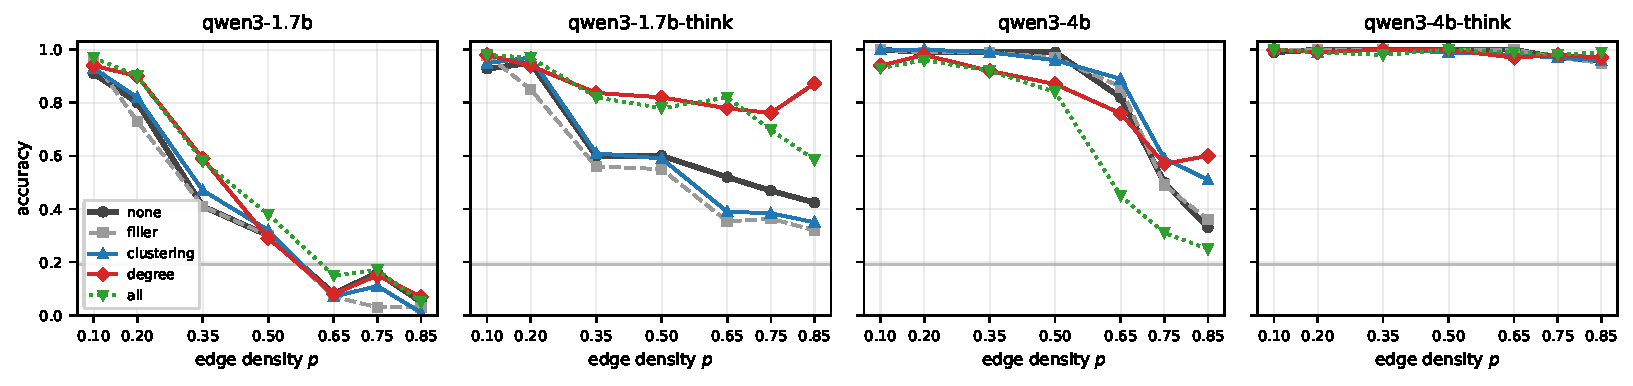
\includegraphics[width=\textwidth]{density.pdf}
\caption{\texttt{node\_degree} accuracy against edge density, all four
arms, five conditions. The grey line is the blind baseline
(Table~\ref{tab:blind}). The panels show why a single pooled number for
``the primer effect'' is not well defined. \texttt{qwen3-1.7b} has a steep
difficulty gradient and admits a positive effect. \texttt{qwen3-4b} is
saturated under \texttt{none} at every density, so the only movement
available is downward. Both thinking arms are at ceiling throughout.
\texttt{degree} and \texttt{all} --- the two conditions that state the
answer --- are the only ones that separate from \texttt{none}, upward at
1.7B and downward at 4B.}
\label{fig:density}
\end{figure*}

Table~\ref{tab:main-results} reports the full sweep and
Figure~\ref{fig:density} the density structure underneath one column of it.
Four observations organize them.

\paragraph{No primer effect replicates across model scale.} Several
(primer, task) cells significantly exceed both \texttt{none} and
\texttt{filler} in one plain arm; none does so in both. The strongest
candidate is the \texttt{degree} primer, and the \texttt{all} primer that
contains it, on \texttt{node\_degree} --- the one task where a primer
states the requested quantity verbatim. It is worth $+7.5$ $[+3.0, +12.0]$
and $+10.2$ $[+5.2, +15.2]$ points to \texttt{qwen3-1.7b}, and $+11.7$ and
$+11.6$ to \texttt{qwen3-1.7b-think}. To \texttt{qwen3-4b} it is worth
$-6.5$ $[-9.2, -4.0]$ and $-9.2$ $[-12.2, -6.2]$, and the 1.7B and 4B
intervals do not overlap in either primer. A primer that \emph{contains the
answer} makes the larger model worse.

The failures are not random. Of \texttt{qwen3-4b}'s $29$ \texttt{degree}
losses, $26$ are off by one to three, and its mean absolute error rises
from $0.015$ under \texttt{none} to $0.138$ under \texttt{degree}. The
primer appears to compete with the model's own enumeration of the
incident-list encoding rather than replace it.

\paragraph{Answer retrieval is partial even where it is complete in
principle.} The shortcut solver attains $1.00$ on \texttt{node\_degree}
under \texttt{degree} and \texttt{all}, and on \texttt{edge\_count} under
the same two primers (Table~\ref{tab:shortcut}). No model arm approaches
that ceiling. The largest \texttt{edge\_count} gain anywhere in the sweep
is \texttt{qwen3-4b} under \texttt{degree} at $+27.7$ points. That takes the
arm from $2.0\%$ to $29.7\%$, still leaving roughly $70\%$ of instances
wrong against a bar of $100\%$. A primer that fully determines the answer
is therefore not a test of graph reasoning, but neither is it automatically
exploited. What it measures is whether the model uses a fact it was handed,
and largely it does not.

\paragraph{The shortcut ceilings do not transfer to this graph size.} They
were fit on GraphQA's native generator, whose graphs have $5$--$19$ nodes.
At the fixed $n{=}40$ used here, the blind baselines of
Table~\ref{tab:blind} dominate them on two tasks: the constant answer
``40'' scores $100\%$ on \texttt{node\_count} and the constant answer
``yes'' scores $100\%$ on \texttt{cycle\_check}, so the tabulated ceilings
understate the trivial baseline for those tasks by a wide margin. Only
ceilings backed by exact theorems --- \texttt{degree} and \texttt{all} on
\texttt{node\_degree} and \texttt{edge\_count} --- carry over unchanged,
and we read ceiling-adjusted effects only on those.

\paragraph{The two controls disagree about which cells are interesting.}
This is worth stating because it is the point of having both.
\texttt{components} is nearly length-free ($39$ characters), so its effects
are content by construction. It is also inert almost everywhere, the
exceptions being \texttt{node\_count} and \texttt{connected\_nodes} at 4B.
\texttt{all}, the longest primer, shows the largest and least consistent
swings --- including $+11.5$ and $-9.8$ on the same task in different model
sizes. Reading either column alone would produce a different account of the
study.

\subsection{Trivially-answerable tasks respond to text, not to structure}
\label{sec:results-nodecount}

The largest effects in Table~\ref{tab:main-results} appear on
\texttt{node\_count}, where the gold answer is the constant $40$
(Table~\ref{tab:blind}) and the question is therefore not a
graph-reasoning question at all. At 1.7B every condition improves over
\texttt{none} ($31.5\%$) by between $+2.0$ and $+67.2$ points, and the
ordering follows no property of primer content: \texttt{clustering}
$+67.2$, \texttt{all} $+47.0$, \texttt{filler} $+39.8$, \texttt{components}
$+21.2$, \texttt{degree} $+6.8$, \texttt{rwse} $+2.0$ (n.s.). At 4B the six
conditions are statistically indistinguishable from one another, all
improving \texttt{none} by $+8.0$ to $+9.8$ points. In both arms the
content-free \texttt{filler} control is among the strongest conditions.

The mechanism is mundane and worth naming. The dominant \texttt{none}
failure is the answer ``$39$'', an off-by-one induced by the encoder's
``nodes $0, \dots, 39$'' listing; the model reports the largest index
rather than the count. Any interposed text appears to disrupt that
reading, and a primer that emits one sentence per node additionally makes
the count recoverable by counting sentences. We accordingly retract the
reading of this cell as a structural primer effect --- an earlier version
of this work reported \texttt{components} on \texttt{node\_count} as a
content gain that replicated across arms, and it does replicate, but so
does \texttt{filler}.

\subsection{Density and the ceiling problem}
\label{sec:results-density}

\begin{table}[t]
\centering
\small
\begin{tabular}{lrrrr}
\toprule
& \multicolumn{4}{c}{density $p$} \\
\cmidrule(lr){2-5}
Condition & $0.10$ & $0.20$ & $0.35$ & $0.50$ \\
\midrule
\multicolumn{5}{l}{\emph{\texttt{qwen3-1.7b}}} \\
\texttt{none}       & 0.910 & 0.800 & 0.410 & 0.300 \\
\texttt{clustering} & 0.930 & 0.820 & 0.470 & 0.320 \\
\texttt{degree}     & 0.940 & 0.900 & 0.590 & 0.290 \\
\texttt{filler}     & 0.960 & 0.730 & 0.410 & 0.300 \\
\texttt{all}        & 0.970 & 0.900 & 0.580 & 0.380 \\
\midrule
\multicolumn{5}{l}{\emph{\texttt{qwen3-4b}}} \\
\texttt{none}       & 1.000 & 0.990 & 0.990 & 0.990 \\
\texttt{clustering} & 1.000 & 1.000 & 0.990 & 0.960 \\
\texttt{degree}     & 0.940 & 0.980 & 0.920 & 0.870 \\
\texttt{filler}     & 1.000 & 0.990 & 0.990 & 0.970 \\
\texttt{all}        & 0.880 & 0.960 & 0.920 & 0.840 \\
\bottomrule
\end{tabular}
\caption{\texttt{node\_degree} accuracy by density, plain arms, selected
conditions; the numbers behind the first two panels of
Figure~\ref{fig:density}.}
\label{tab:density}
\end{table}

Table~\ref{tab:density} shows why the sign reversal above is not a
contradiction but a ceiling artifact. \texttt{qwen3-4b} answers
\texttt{node\_degree} correctly on $99\%$ of instances under \texttt{none}
at every density in the sweep. The task supplies no headroom in which a
primer could help, so the only measurable effect is the cost of the added
tokens. \texttt{qwen3-1.7b} degrades from $0.910$ to $0.300$ over the same
range and does admit a positive effect.

This generalizes beyond the one task. A cell that is saturated for one
model and taxing for another cannot yield a model-independent primer
effect, and an estimate pooled over the two arms averages a ceiling against
a floor. Of the $24$ (arm, task) cells in Table~\ref{tab:main-results}, $10$
sit at or above $98\%$ under \texttt{none} and therefore admit no upward
effect at all; $2$ are censored past interpretability
(Section~\ref{sec:results-truncation}); and $2$ more have effectively
constant gold answers. The design question a primer study has to answer
before measuring anything is which cells are left.

\subsection{Prompt length is not a neutral covariate}
\label{sec:results-length}

The \texttt{filler} condition is not inert. It significantly harms
\texttt{qwen3-1.7b} on \texttt{edge\_existence} ($-15.8$ $[-20.0, -11.8]$)
and \texttt{connected\_nodes} ($-6.2$ $[-10.2, -2.2]$), and
\texttt{qwen3-4b} on \texttt{connected\_nodes} ($-12.5$ $[-17.0, -8.0]$)
and \texttt{edge\_existence} ($-7.0$ $[-10.8, -3.5]$), while significantly
\emph{helping} both arms on the trivially-answerable \texttt{node\_count}.
It carries no structural information by construction, so any effect it
registers is attributable to length and position alone
\citep{liu2024lostinthemiddle,kamradt2023needle}. Effects of comparable
magnitude measured against \texttt{none} for the informative primers
therefore cannot be credited to content without this control.

\begin{table}[t]
\centering
\small
\begin{tabular}{lrrr}
\toprule
$p$ & $n$ & $\Delta$ & $p$-value \\
\midrule
0.10 & 390 & $+2.3$ & 0.078 \\
0.20 & 397 & $+2.5$ & 0.174 \\
0.35 & 399 & $-4.3$ & 0.107 \\
0.50 & 400 & $-9.5$ & 0.0002 \\
0.65 & 399 & $-9.3$ & 0.0007 \\
0.75 & 397 & $-14.1$ & $<10^{-4}$ \\
0.85 & 392 & $-11.7$ & 0.0001 \\
\midrule
pooled & 2774 & $-6.3$ & $<10^{-4}$ \\
\bottomrule
\end{tabular}
\caption{The length effect in isolation: \texttt{filler} against
\texttt{none} on \texttt{node\_degree}, \texttt{qwen3-1.7b-think}, over a
wider density range than the main sweep. $\Delta$ in percentage points.
Content-free text is harmless on sparse graphs and costs up to $14.1$
points on dense ones --- more than most primer \emph{contents} gain
anywhere in this study.}
\label{tab:filler}
\end{table}

Table~\ref{tab:filler} bounds the confound directly. The effect is not
constant: filler is harmless, even mildly helpful, at $p \le 0.20$, and
turns sharply negative from $p = 0.50$ upward. That shape matters for
reading the main sweep, whose densest level is $0.50$: the length penalty
there is real but near the bottom of its range, so
Table~\ref{tab:main-results} understates how much of a long primer's effect
is length rather than content.

\subsection{Chain-of-thought dominates every primer effect}
\label{sec:results-cot}

\begin{table}[t]
\centering
\small
\begin{tabular}{lrrrr}
\toprule
$p$ & $n$ & plain & think & $\Delta$ \\
\midrule
0.10 & 1185 & 0.929 & 0.958 & $+2.9$ \\
0.20 & 1196 & 0.781 & 0.901 & $+12.0$ \\
0.35 & 1199 & 0.425 & 0.655 & $+22.9$ \\
0.50 & 1200 & 0.292 & 0.581 & $+28.8$ \\
0.65 & 1552 & 0.126 & 0.503 & $+37.7$ \\
0.75 & 1554 & 0.094 & 0.476 & $+38.2$ \\
0.85 & 1553 & 0.054 & 0.554 & $+50.0$ \\
\midrule
pooled & 9439 & 0.318 & 0.610 & $+29.2$ \\
\bottomrule
\end{tabular}
\caption{Chain-of-thought against greedy decoding on the identical
\texttt{qwen3-1.7b} checkpoint and byte-identical prompts,
\texttt{node\_degree}, pooled over the \texttt{none}, \texttt{components},
\texttt{clustering} and \texttt{degree} conditions. $\Delta$ in percentage
points; every level significant at $p < 10^{-3}$ under an exact McNemar
test, the pooled comparison beyond the range of exact computation
($z = 46.4$).}
\label{tab:cot}
\end{table}

Table~\ref{tab:cot} isolates the reasoning-mode effect from the primer
channel: same checkpoint, same prompts, decoding mode alone. It is worth
$+29.2$ points pooled and $+50.0$ points at $p = 0.85$ --- an order of
magnitude above the largest primer effect in Table~\ref{tab:main-results}
that is not answer retrieval, and consistent with
\citet{wei2022chainofthought}. Note also that it grows with density while
the primer effects do not, which is what one expects of an intervention
that adds computation rather than information.

The consequence for this study is visible in the last two blocks of
Table~\ref{tab:main-results}. The thinking arms are at ceiling on
\texttt{cycle\_check}, \texttt{edge\_existence} and \texttt{node\_count}
under every condition, and \texttt{qwen3-4b-think} on five of six tasks.
No headroom remains in which a primer effect could be observed.
Where chain-of-thought does not saturate a task it censors it instead
(Section~\ref{sec:results-truncation}). A primer study conducted only on
reasoning-mode models of this scale would have almost no interpretable
cells to report at all.

Primers do, however, change how often the thinking arms fail to terminate
--- an effect on the \emph{process} rather than on accuracy, and one that
would be invisible to an accuracy-only analysis. For
\texttt{qwen3-1.7b-think}, \texttt{degree} truncates $3.4$ points more
often than \texttt{none} ($p < 0.001$) while \texttt{all} ($-3.4$),
\texttt{filler} ($-1.8$) and \texttt{clustering} ($-1.3$) truncate less;
for \texttt{qwen3-4b-think}, every primer truncates less than
\texttt{none}, by $2.0$ to $4.3$ points (all $p < 0.001$). A primer
therefore changes how long the model thinks even where it does not change
what the model concludes.

\subsection{The one cell that survives every control}
\label{sec:results-headline}

\begin{table}[t]
\centering
\small
\begin{tabular}{lrrcr}
\toprule
Sample & $\Delta$ & $n$ & 95\% CI & $p$ \\
\midrule
\multicolumn{5}{l}{\emph{Original sample}} \\
$p=0.10$    & $+0.3$ & 400 & --- & 1.000 \\
$p=0.20$    & $+3.3$ & 400 & --- & 0.182 \\
$p=0.35$    & $+7.5$ & 400 & --- & 0.009 \\
$p=0.50$    & $+4.3$ & 400 & --- & 0.155 \\
pooled      & $+3.8$ & 1600 & $[+1.5, +6.2]$ & 0.0017 \\
\midrule
\multicolumn{5}{l}{\emph{Replication, independent graphs}} \\
$p=0.10$    & $+2.0$ & 400 & --- & 0.185 \\
$p=0.20$    & $+4.0$ & 400 & --- & 0.101 \\
$p=0.35$    & $+4.5$ & 400 & --- & 0.145 \\
$p=0.50$    & $+6.5$ & 400 & --- & 0.028 \\
pooled      & $+4.3$ & 1600 & $[+1.9, +6.6]$ & 0.0006 \\
\bottomrule
\end{tabular}
\caption{\texttt{qwen3-1.7b}, \texttt{node\_degree}, \texttt{clustering}
against \texttt{none}, $n{=}40$, $400$ paired instances per density level.
$\Delta$ in percentage points; $p$ from the exact McNemar test
(permutation $p$ pooled: $0.0015$ and $0.0007$). Per-level rows are
descriptive and are a family of four --- none survives correction on its
own, which is the expected picture for an effect of this size at $400$
pairs. The effect is positive at every level in both samples, which eight
independent coin flips would produce with probability $1/256$.}
\label{tab:headline}
\end{table}

One cell clears every control applied in this study, and we report it
separately because the power available to it is four times that of any
single cell in Table~\ref{tab:main-results}. On a dedicated sweep of $400$
graphs per density level, the \texttt{clustering} primer improves
\texttt{qwen3-1.7b} on \texttt{node\_degree} by $+3.8$ points $[+1.5,
+6.2]$, and an independent sample at the same design points reproduces it
at $+4.3$ points $[+1.9, +6.6]$; see Table~\ref{tab:headline}.

The effect survives each control in turn. It is not answer leakage: the
shortcut ceiling for \texttt{clustering} on \texttt{node\_degree} is
$0.082$ (Table~\ref{tab:shortcut}), the same as \texttt{none}, because a
clustering coefficient does not determine a degree. It is not length:
\texttt{clustering} is $200$ characters \emph{shorter} than the
null-content \texttt{filler} (Table~\ref{tab:lengths}), which registers no
effect on this task in either 1.7B arm ($-0.5$ and $-3.5$, both n.s.). And
it is not a single lucky density level: it is positive at all four in both
samples.

We are nonetheless cautious about it, for three reasons. The main sweep is
consistent with it but cannot confirm it: at $100$ graphs per cell it
measures $+3.0$ points ($p = 0.256$), which is what a fourfold reduction in
sample size predicts for an effect of this magnitude, not a failed
replication. Under chain-of-thought the corresponding estimates are $+1.0$
($p = 0.694$) in the main sweep and $-1.1$ ($p = 0.244$) on the
wide-density sweep, so the effect does not survive into the thinking arm.
And \texttt{qwen3-4b} cannot test it at all, being saturated under
\texttt{none} (Table~\ref{tab:density}). We therefore report it as a
single, replicated, model- and mode-specific effect, not as a general
property of clustering primers.

For completeness: \texttt{components} was tested on the same original
sweep and is inert pooled ($+0.1$ points, $p = 0.948$), but its paired
difference trends negative with density (slope $-0.148$ per unit density,
permutation $p = 0.022$), driven by $-5.0$ points at $p=0.50$. We do not
interpret this --- it is one slope out of a small family --- but record it
because \texttt{components} is the one condition whose effects cannot be
length.

\subsection{Sensitivity to the truncation convention}
\label{sec:results-sensitivity}

\begin{table}[t]
\centering
\small
\begin{tabular}{lrr}
\toprule
& \multicolumn{2}{c}{$\Delta$ vs \texttt{none}} \\
\cmidrule(lr){2-3}
Primer & dropped & zeroed \\
\midrule
\texttt{rwse}       & $\mathbf{-7.5}$ & $-0.2$ \\
\texttt{clustering} & $+0.3$ & $\mathbf{+8.5}$ \\
\texttt{all}        & $-1.1$ & $\mathbf{+7.0}$ \\
\bottomrule
\end{tabular}
\caption{Where the two conventions for truncated generations disagree, on
\texttt{qwen3-1.7b} / \texttt{cycle\_check}.
Dropping the pair (this paper) and scoring it incorrect
(\texttt{check\_significance.py}) give opposite verdicts on 1.7B
\texttt{cycle\_check}, because \texttt{none} truncates on $9\%$ of that
task's rows while \texttt{clustering} and \texttt{all} truncate on under
$1\%$. Neither convention is uniformly more conservative; both are reported
so the disagreement is visible rather than buried in a pipeline choice.}
\label{tab:sensitivity}
\end{table}

Excluding truncated generations rather than scoring them incorrect is a
choice, and on two tasks it changes the verdict rather than the third
decimal place. Table~\ref{tab:sensitivity} gives the case where it matters
most. Under the drop convention \texttt{rwse} costs 1.7B $7.5$ points on
\texttt{cycle\_check}; under the zero convention that effect vanishes and
two others appear, because the arms being compared truncate at very
different rates. The drop convention answers ``given that both arms
produced an answer, which was right more often?''; the zero convention
answers ``which arm produced a correct answer more often?''. Both are
legitimate, and a primer that makes a model ramble until it runs out of
budget has caused a real failure that the drop convention forgives. We use
the drop convention throughout and report the disagreement here; on every
task other than \texttt{cycle\_check} and \texttt{edge\_count} the two
agree, because truncation is under $1\%$.

\section{Discussion}
\label{sec:discussion}

The central negative result of this study is a failure to replicate across
scale: of the $144$ (arm, task, primer) comparisons in
Table~\ref{tab:main-results}, no primer effect that clears both the
\texttt{none} baseline and the \texttt{filler} control in one model size
does so in the other. Three regularities account for most of what the table
contains, and none of them is the mechanism a primer was hypothesized to
supply.

First, a primer helps reliably only where it states the requested quantity
verbatim, and even then only partially. \texttt{degree} and \texttt{all}
move \texttt{node\_degree} and \texttt{edge\_count} and move nothing else
consistently; the derived statistics that do not name an answer ---
\texttt{clustering}, \texttt{rwse}, \texttt{components} --- produce no
effect that survives both controls in more than one arm. This is answer
retrieval, the behaviour the shortcut solver was built to expose, and the
models perform it badly: never more than $28$ points of a $100$-point
available gain on \texttt{edge\_count}, and at 4B in the wrong direction
entirely. The natural reading is that a primer does not replace the
model's own computation but competes with it, and that the model with the
better internal computation has more to lose.

Second, added text is an active treatment regardless of its content. The
length-matched \texttt{filler} significantly harms both model sizes on
\texttt{edge\_existence} and \texttt{connected\_nodes} and significantly
helps both on \texttt{node\_count}, at magnitudes ($-15.8$ to $+39.8$
points) exceeding nearly every content effect measured here. An
experimental design that compares a primer only against \texttt{none} ---
the design a naive reading of the primer hypothesis invites --- therefore
estimates content and length confounded, with the length term frequently
the larger of the two. We would go further: a primer paper reporting gains
against a no-primer baseline alone should be assumed to be reporting a
length effect until a placebo says otherwise.

Third, the headroom in which any of this could be measured is largely
consumed by the decoding mode. Chain-of-thought is worth $+29.2$ points
pooled on an identical checkpoint (Table~\ref{tab:cot}), and its effect is
to move most (task, arm) cells to ceiling: \texttt{qwen3-4b-think} exceeds
$97\%$ accuracy under \texttt{none} on five of six tasks, and on those five
no primer differs from \texttt{none} by more than $1$ point. Where
chain-of-thought does not saturate a task it censors it instead: the
$62$--$81\%$ truncation rate on \texttt{edge\_count}
(Table~\ref{tab:hitcap}) removes that task from analysis in both thinking
arms. A primer study conducted only on reasoning-mode models of this scale
would have almost no interpretable cells to report.

Taken together, these results argue that the interesting quantity is not
whether a structural preamble helps, but where it \emph{could} help. Of the
$24$ (arm, task) cells in Table~\ref{tab:main-results}, $10$ are at or above
$98\%$ under \texttt{none} and therefore admit no upward effect, $2$ are
censored past interpretability, and $2$ more (\texttt{node\_count},
\texttt{cycle\_check}) have effectively constant gold answers at this graph
size and measure response formatting rather than graph reasoning. The cells
that remain are few enough to enumerate, and they are the ones on which the
replicated \texttt{clustering} effect of Table~\ref{tab:headline} was
found. Screening for interpretable cells before measuring, rather than
measuring everywhere and interpreting afterwards, is the design lesson we
would carry forward.

\section{Conclusion}
\label{sec:conclusion}

We evaluated seven primer conditions across six GraphQA tasks, four
densities and four model arms at $n{=}40$, a total of $67{,}200$
generations. Two controls a primer study needs and rarely has bound the
result: a graph-blind solver measuring how much of an effect is answer
retrieval, and a length-matched, content-free primer measuring how much is
prompt length. No primer effect clears both controls in both model sizes.
The effects that do appear are of two kinds. Some are retrieval of a stated
answer, which the models exploit only partially and which reverses sign at
4B; the rest are responses to added text irrespective of its content. One
exception survives every control and an independent replication:
\texttt{clustering} on \texttt{node\_degree} for \texttt{qwen3-1.7b}, $+3.8$
and $+4.3$ points. We read the broader result not as evidence that
structural preambles cannot help, but that most (model, task) pairs at this
scale afford no interpretable test of whether they do.

\section*{Limitations}
\label{sec:limitations}

This sweep covers only two model sizes (1.7B and 4B parameters) from a
single model family, so the findings may not generalize to substantially
larger models or to other architectures. The direction of the
\texttt{degree} effect reverses between the two sizes we do have, which is
a reason to expect further reversals rather than a stable trend.

Several (primer condition, task) cells are known in advance to be
shortcut-dominated at this graph size and density range
(Section~\ref{sec:setup}); results on those cells bound what can be
concluded about genuine graph reasoning even though we report them.

Graphs are drawn from a single generator family (Erd\H{o}s--R\'enyi).
Whether primer effects transfer to other generators remains untested,
and \citet{fatemi2023talklikeagraph} show the generator matters for
encoding effects. As noted in Section~\ref{sec:related-work}, varying the
generator family is not itself a safe way to test this: it confounds
structure with task difficulty.

Compute and time constraints limited this sweep to a single
node-count/density design rather than a broader sweep over graph sizes. All
results are at $n{=}40$, and the shortcut ceilings were fit at $n \le 19$,
so the one number we carry across sizes is the one we flag as not
transferring.

Finally, the length control is a bracket rather than an exact match: the
\texttt{filler} condition is longer than \texttt{degree} and
\texttt{clustering} and shorter than \texttt{rwse} and \texttt{all}
(Table~\ref{tab:lengths}), so it bounds the length term without
eliminating it. A design holding rendered length exactly constant while
varying structure would isolate content more sharply than subtracting a
bracketing control, and we regard that as the natural next step.

\section*{Ethics Statement}

This work evaluates open-weight language models on synthetically generated
Erd\H{o}s--R\'enyi graphs. It involves no human subjects, no personal or
identifying data, and no annotation labour: gold answers are computed
programmatically from the graphs rather than collected from people. We see
no direct risk of harm arising from the findings, which are a negative
result about a prompting technique. The principal societal cost is the
compute expended, reported in Section~\ref{sec:setup}.

\bibliography{custom}

\appendix

\section{Effect sizes with confidence intervals, all cells}
\label{sec:appendix-ci}

Paired effect sizes for every (arm, task, primer) cell: $\Delta$ in
percentage points against \texttt{none}, an exact $95\%$ interval
conditional on the discordant pairs (Clopper--Pearson, inverting the
same exact McNemar test used for the per-cell $p$-values), the
permutation $p$-value, and $\Delta$ under the alternative
convention that scores truncated generations incorrect rather than
dropping the pair (Section~\ref{sec:extraction}). $n$ is the
number of pairs in which neither arm truncated. ``n/a'' marks a cell
in which no pair disagreed: the conditional estimate is then exactly
zero with no width, which is a statement about this sample and not a
bound on the effect, so the discordant count is reported instead.

\begin{table}[H]
\centering\footnotesize
\setlength{\tabcolsep}{3pt}
\resizebox{\columnwidth}{!}{%
\begin{tabular}{llrrrrr}
\toprule
Task & Primer & $n$ & $\Delta$ & 95\% CI & perm $p$ & zeroed \\
\midrule
\texttt{connected\_nodes} & components & 400 & $+0.8$ & $[-3.1, +4.5]$ & 0.7861 & $+0.8$ \\
 & clustering & 400 & $+1.2$ & $[-3.3, +5.7]$ & 0.6458 & $+1.2$ \\
 & rwse & 400 & $+1.0$ & $[-3.5, +5.5]$ & 0.7304 & $+1.0$ \\
 & degree & 400 & $+3.5$ & $[-0.8, +7.5]$ & 0.1239 & $+3.5$ \\
 & filler & 400 & $-6.2$ & $[-10.0, -1.9]$ & 0.0040 & $-6.2$ \\
 & all & 399 & $+2.0$ & $[-2.9, +6.8]$ & 0.4644 & $+2.0$ \\
\midrule
\texttt{cycle\_check} & components & 343 & $-0.6$ & $[-0.6, +0.4]$ & 0.5033 & $+2.0$ \\
 & clustering & 362 & $+0.3$ & $[-0.3, +0.3]$ & 1.0000 & $+8.5$ \\
 & rwse & 358 & $-7.5$ & $[-8.1, -5.2]$ & 0.0001 & $-0.2$ \\
 & degree & 301 & $-12.6$ & $[-12.6, -10.3]$ & 0.0001 & $-17.5$ \\
 & filler & 341 & $+0.3$ & $[-0.3, +0.3]$ & 1.0000 & $+3.0$ \\
 & all & 362 & $-1.1$ & $[-1.6, +0.5]$ & 0.2210 & $+7.0$ \\
\midrule
\texttt{edge\_count} & components & 211 & $-1.4$ & $[-2.3, +1.0]$ & 0.3783 & $-1.0$ \\
 & clustering & 238 & $-0.4$ & $[-2.4, +1.9]$ & 1.0000 & $-0.5$ \\
 & rwse & 239 & $-0.8$ & $[-2.3, +1.4]$ & 0.6837 & $-0.8$ \\
 & degree & 253 & $+4.0$ & $[+0.6, +5.8]$ & 0.0179 & $+3.0$ \\
 & filler & 224 & $-0.4$ & $[-2.0, +1.6]$ & 1.0000 & $-0.5$ \\
 & all & 211 & $+2.4$ & $[-1.1, +4.6]$ & 0.2269 & $+0.8$ \\
\midrule
\texttt{edge\_existence} & components & 400 & $-8.2$ & $[-10.9, -4.7]$ & 0.0001 & $-8.2$ \\
 & clustering & 400 & $+3.8$ & $[-0.9, +8.1]$ & 0.1199 & $+3.8$ \\
 & rwse & 399 & $+5.3$ & $[+0.4, +9.8]$ & 0.0321 & $+5.0$ \\
 & degree & 400 & $+4.0$ & $[-0.7, +8.4]$ & 0.0957 & $+4.0$ \\
 & filler & 400 & $-15.8$ & $[-18.3, -12.0]$ & 0.0001 & $-15.8$ \\
 & all & 400 & $+11.5$ & $[+6.5, +15.8]$ & 0.0001 & $+11.5$ \\
\midrule
\texttt{node\_count} & components & 400 & $+21.2$ & $[+15.9, +25.6]$ & 0.0001 & $+21.2$ \\
 & clustering & 400 & $+67.2$ & $[+65.4, +67.2]$ & 0.0001 & $+67.2$ \\
 & rwse & 400 & $+2.0$ & $[-4.5, +8.5]$ & 0.5871 & $+2.0$ \\
 & degree & 400 & $+6.8$ & $[+2.9, +9.9]$ & 0.0008 & $+6.8$ \\
 & filler & 400 & $+39.8$ & $[+37.2, +40.6]$ & 0.0001 & $+39.8$ \\
 & all & 400 & $+47.0$ & $[+43.8, +48.7]$ & 0.0001 & $+47.0$ \\
\midrule
\texttt{node\_degree} & components & 400 & $+1.8$ & $[-2.4, +5.8]$ & 0.4599 & $+1.8$ \\
 & clustering & 400 & $+3.0$ & $[-2.0, +7.8]$ & 0.2577 & $+3.0$ \\
 & rwse & 399 & $+4.0$ & $[-0.9, +8.6]$ & 0.1104 & $+4.0$ \\
 & degree & 400 & $+7.5$ & $[+2.8, +11.6]$ & 0.0018 & $+7.5$ \\
 & filler & 400 & $-0.5$ & $[-4.6, +3.7]$ & 0.9028 & $-0.5$ \\
 & all & 400 & $+10.2$ & $[+4.9, +15.0]$ & 0.0003 & $+10.2$ \\
\bottomrule
\end{tabular}}
\caption{\texttt{qwen3-1.7b}: all cells.}
\end{table}

\begin{table}[H]
\centering\footnotesize
\setlength{\tabcolsep}{3pt}
\resizebox{\columnwidth}{!}{%
\begin{tabular}{llrrrrr}
\toprule
Task & Primer & $n$ & $\Delta$ & 95\% CI & perm $p$ & zeroed \\
\midrule
\texttt{connected\_nodes} & components & 392 & $+2.8$ & $[-0.7, +5.9]$ & 0.1268 & $+2.5$ \\
 & clustering & 394 & $+1.5$ & $[-2.7, +5.6]$ & 0.5384 & $+2.0$ \\
 & rwse & 393 & $-0.3$ & $[-4.3, +3.8]$ & 1.0000 & $+0.2$ \\
 & degree & 390 & $+7.4$ & $[+3.5, +10.6]$ & 0.0001 & $+6.2$ \\
 & filler & 394 & $+2.0$ & $[-1.7, +5.5]$ & 0.3275 & $+2.5$ \\
 & all & 392 & $+6.1$ & $[+2.2, +9.4]$ & 0.0027 & $+6.2$ \\
\midrule
\texttt{cycle\_check} & components & 346 & $+0.0$ & n/a ($0$ disc.) & 1.0000 & $-7.5$ \\
 & clustering & 376 & $+0.0$ & n/a ($0$ disc.) & 1.0000 & $-0.5$ \\
 & rwse & 386 & $+0.0$ & n/a ($0$ disc.) & 1.0000 & $+2.2$ \\
 & degree & 295 & $-0.7$ & $[-0.7, +0.5]$ & 0.5036 & $-21.8$ \\
 & filler & 388 & $+0.0$ & n/a ($0$ disc.) & 1.0000 & $+3.0$ \\
 & all & 373 & $+0.0$ & n/a ($0$ disc.) & 1.0000 & $-0.8$ \\
\midrule
\texttt{edge\_count} & components & 27 & $+7.4$ & $[-5.1, +7.4]$ & 0.5037 & $-0.8$ \\
 & clustering & 23 & $-8.7$ & $[-17.2, +10.6]$ & 0.6251 & $-1.2$ \\
 & rwse & 25 & $-4.0$ & $[-4.0, +3.8]$ & 1.0000 & $-3.2$ \\
 & degree & 13 & $-61.5$ & $[-61.5, -16.1]$ & 0.0102 & $-3.2$ \\
 & filler & 29 & $+3.4$ & $[-8.4, +10.2]$ & 1.0000 & $-1.5$ \\
 & all & 24 & $-8.3$ & $[-22.8, +13.9]$ & 0.6794 & $+5.0$ \\
\midrule
\texttt{edge\_existence} & components & 398 & $-0.8$ & $[-1.9, +0.9]$ & 0.5090 & $-0.8$ \\
 & clustering & 398 & $-1.0$ & $[-1.9, +0.6]$ & 0.2911 & $-1.0$ \\
 & rwse & 398 & $-1.3$ & $[-2.4, +0.6]$ & 0.2274 & $-1.2$ \\
 & degree & 397 & $-2.3$ & $[-3.1, -0.3]$ & 0.0249 & $-2.5$ \\
 & filler & 399 & $-0.8$ & $[-1.9, +0.9]$ & 0.5051 & $-0.5$ \\
 & all & 399 & $-2.0$ & $[-2.9, -0.1]$ & 0.0374 & $-1.8$ \\
\midrule
\texttt{node\_count} & components & 342 & $+0.9$ & $[-0.6, +1.4]$ & 0.3758 & $+1.5$ \\
 & clustering & 369 & $+1.4$ & $[-0.1, +1.4]$ & 0.0597 & $+9.0$ \\
 & rwse & 369 & $+1.4$ & $[-0.1, +1.4]$ & 0.0597 & $+9.0$ \\
 & degree & 360 & $+0.8$ & $[-0.8, +1.8]$ & 0.4512 & $+5.5$ \\
 & filler & 369 & $+1.4$ & $[-0.1, +1.4]$ & 0.0597 & $+9.0$ \\
 & all & 369 & $+1.4$ & $[-0.1, +1.4]$ & 0.0597 & $+9.0$ \\
\midrule
\texttt{node\_degree} & components & 395 & $-1.0$ & $[-4.4, +2.6]$ & 0.6543 & $-1.0$ \\
 & clustering & 396 & $+1.0$ & $[-3.0, +4.9]$ & 0.7010 & $+1.5$ \\
 & rwse & 394 & $+2.5$ & $[-1.9, +6.8]$ & 0.2898 & $+2.5$ \\
 & degree & 376 & $+11.7$ & $[+7.4, +15.0]$ & 0.0001 & $+8.8$ \\
 & filler & 396 & $-3.5$ & $[-7.3, +0.6]$ & 0.0954 & $-3.0$ \\
 & all & 396 & $+11.6$ & $[+7.3, +15.0]$ & 0.0001 & $+12.2$ \\
\bottomrule
\end{tabular}}
\caption{\texttt{qwen3-1.7b-think}: all cells.}
\end{table}

\begin{table}[H]
\centering\footnotesize
\setlength{\tabcolsep}{3pt}
\resizebox{\columnwidth}{!}{%
\begin{tabular}{llrrrrr}
\toprule
Task & Primer & $n$ & $\Delta$ & 95\% CI & perm $p$ & zeroed \\
\midrule
\texttt{connected\_nodes} & components & 400 & $+9.2$ & $[+6.1, +11.3]$ & 0.0001 & $+9.2$ \\
 & clustering & 400 & $+1.0$ & $[-3.1, +5.0]$ & 0.6893 & $+1.0$ \\
 & rwse & 400 & $+0.0$ & $[-4.2, +4.2]$ & 1.0000 & $+0.0$ \\
 & degree & 400 & $-3.0$ & $[-7.1, +1.4]$ & 0.1882 & $-3.0$ \\
 & filler & 400 & $-12.5$ & $[-16.2, -7.9]$ & 0.0001 & $-12.5$ \\
 & all & 400 & $-2.8$ & $[-7.0, +1.7]$ & 0.2511 & $-2.8$ \\
\midrule
\texttt{cycle\_check} & components & 391 & $-1.3$ & $[-1.8, +0.3]$ & 0.1318 & $-2.0$ \\
 & clustering & 395 & $+0.3$ & $[-0.2, +0.3]$ & 1.0000 & $+0.5$ \\
 & rwse & 392 & $+0.3$ & $[-0.2, +0.3]$ & 1.0000 & $-0.2$ \\
 & degree & 391 & $-1.5$ & $[-1.5, -0.1]$ & 0.0312 & $-2.2$ \\
 & filler & 392 & $-0.3$ & $[-0.3, +0.2]$ & 1.0000 & $-0.5$ \\
 & all & 395 & $-0.5$ & $[-1.0, +0.6]$ & 0.6269 & $-0.2$ \\
\midrule
\texttt{edge\_count} & components & 397 & $-1.3$ & $[-2.1, +0.5]$ & 0.1756 & $-1.2$ \\
 & clustering & 399 & $-1.3$ & $[-2.4, +0.6]$ & 0.2298 & $-1.2$ \\
 & rwse & 398 & $-1.5$ & $[-2.0, +0.1]$ & 0.0668 & $-1.5$ \\
 & degree & 393 & $+27.7$ & $[+24.5, +29.4]$ & 0.0001 & $+27.3$ \\
 & filler & 400 & $+1.2$ & $[-0.9, +2.9]$ & 0.3012 & $+1.2$ \\
 & all & 397 & $+3.8$ & $[+1.1, +5.6]$ & 0.0049 & $+3.8$ \\
\midrule
\texttt{edge\_existence} & components & 400 & $-2.8$ & $[-5.8, +0.7]$ & 0.1254 & $-2.8$ \\
 & clustering & 400 & $+4.0$ & $[+0.7, +6.7]$ & 0.0168 & $+4.0$ \\
 & rwse & 400 & $-10.0$ & $[-12.9, -6.2]$ & 0.0001 & $-10.0$ \\
 & degree & 398 & $-4.3$ & $[-7.3, -0.7]$ & 0.0200 & $-4.8$ \\
 & filler & 400 & $-7.0$ & $[-10.0, -3.3]$ & 0.0002 & $-7.0$ \\
 & all & 399 & $-9.8$ & $[-12.9, -5.8]$ & 0.0001 & $-10.0$ \\
\midrule
\texttt{node\_count} & components & 400 & $+9.0$ & $[+6.9, +9.5]$ & 0.0001 & $+9.0$ \\
 & clustering & 400 & $+8.8$ & $[+6.2, +9.9]$ & 0.0001 & $+8.8$ \\
 & rwse & 400 & $+9.2$ & $[+6.9, +10.1]$ & 0.0001 & $+9.2$ \\
 & degree & 400 & $+8.0$ & $[+5.1, +9.7]$ & 0.0001 & $+8.0$ \\
 & filler & 400 & $+9.2$ & $[+7.5, +9.2]$ & 0.0001 & $+9.2$ \\
 & all & 400 & $+9.8$ & $[+8.0, +9.8]$ & 0.0001 & $+9.8$ \\
\midrule
\texttt{node\_degree} & components & 400 & $+0.2$ & $[-0.2, +0.2]$ & 1.0000 & $+0.2$ \\
 & clustering & 400 & $-0.5$ & $[-1.7, +1.0]$ & 0.7246 & $-0.5$ \\
 & rwse & 400 & $-2.2$ & $[-3.1, -0.3]$ & 0.0240 & $-2.2$ \\
 & degree & 400 & $-6.5$ & $[-7.7, -4.0]$ & 0.0001 & $-6.5$ \\
 & filler & 400 & $-0.5$ & $[-1.7, +1.0]$ & 0.7232 & $-0.5$ \\
 & all & 400 & $-8.0$ & $[-8.9, -5.6]$ & 0.0001 & $-8.0$ \\
\bottomrule
\end{tabular}}
\caption{\texttt{qwen3-4b}: all cells.}
\end{table}

\begin{table}[H]
\centering\footnotesize
\setlength{\tabcolsep}{3pt}
\resizebox{\columnwidth}{!}{%
\begin{tabular}{llrrrrr}
\toprule
Task & Primer & $n$ & $\Delta$ & 95\% CI & perm $p$ & zeroed \\
\midrule
\texttt{connected\_nodes} & components & 377 & $+0.5$ & $[-0.6, +1.0]$ & 0.6249 & $+0.5$ \\
 & clustering & 373 & $+0.0$ & $[-1.2, +1.2]$ & 1.0000 & $-0.8$ \\
 & rwse & 379 & $+0.0$ & $[-1.4, +1.4]$ & 1.0000 & $+0.5$ \\
 & degree & 376 & $+0.0$ & $[-1.5, +1.5]$ & 1.0000 & $+0.5$ \\
 & filler & 379 & $+0.8$ & $[-0.6, +1.3]$ & 0.3787 & $+1.2$ \\
 & all & 375 & $-0.5$ & $[-1.8, +1.1]$ & 0.7306 & $-1.2$ \\
\midrule
\texttt{cycle\_check} & components & 381 & $+0.0$ & n/a ($0$ disc.) & 1.0000 & $-3.2$ \\
 & clustering & 394 & $+0.0$ & n/a ($0$ disc.) & 1.0000 & $+0.0$ \\
 & rwse & 395 & $+0.0$ & n/a ($0$ disc.) & 1.0000 & $+0.2$ \\
 & degree & 375 & $-0.8$ & $[-0.8, +0.3]$ & 0.2514 & $-5.5$ \\
 & filler & 396 & $+0.0$ & n/a ($0$ disc.) & 1.0000 & $+0.5$ \\
 & all & 392 & $+0.0$ & n/a ($0$ disc.) & 1.0000 & $-0.5$ \\
\midrule
\texttt{edge\_count} & components & 60 & $+1.7$ & $[-1.6, +1.7]$ & 1.0000 & $+24.8$ \\
 & clustering & 59 & $+1.7$ & $[-4.1, +5.0]$ & 1.0000 & $+24.8$ \\
 & rwse & 49 & $+0.0$ & $[-4.0, +4.0]$ & 1.0000 & $+10.2$ \\
 & degree & 34 & $-23.5$ & $[-23.5, -6.1]$ & 0.0073 & $+8.5$ \\
 & filler & 50 & $-2.0$ & $[-2.0, +1.9]$ & 1.0000 & $+12.2$ \\
 & all & 41 & $-41.5$ & $[-41.5, -25.3]$ & 0.0002 & $+1.8$ \\
\midrule
\texttt{edge\_existence} & components & 396 & $+0.0$ & n/a ($0$ disc.) & 1.0000 & $-0.5$ \\
 & clustering & 396 & $+0.0$ & n/a ($0$ disc.) & 1.0000 & $-0.8$ \\
 & rwse & 393 & $+0.0$ & n/a ($0$ disc.) & 1.0000 & $-1.2$ \\
 & degree & 398 & $+0.0$ & n/a ($0$ disc.) & 1.0000 & $+0.0$ \\
 & filler & 399 & $+0.0$ & n/a ($0$ disc.) & 1.0000 & $+0.0$ \\
 & all & 394 & $+0.0$ & n/a ($0$ disc.) & 1.0000 & $-1.0$ \\
\midrule
\texttt{node\_count} & components & 400 & $+0.0$ & $[-0.9, +0.9]$ & 1.0000 & $+0.0$ \\
 & clustering & 399 & $+0.5$ & $[-0.3, +0.5]$ & 0.4936 & $+0.2$ \\
 & rwse & 399 & $+0.5$ & $[-0.3, +0.5]$ & 0.5005 & $+0.2$ \\
 & degree & 399 & $+0.5$ & $[-0.3, +0.5]$ & 0.5005 & $+0.2$ \\
 & filler & 400 & $+0.5$ & $[-0.3, +0.5]$ & 0.4870 & $+0.5$ \\
 & all & 400 & $+0.5$ & $[-0.3, +0.5]$ & 0.4870 & $+0.5$ \\
\midrule
\texttt{node\_degree} & components & 380 & $-0.3$ & $[-0.3, +0.3]$ & 1.0000 & $+0.2$ \\
 & clustering & 386 & $-0.3$ & $[-0.8, +0.6]$ & 1.0000 & $+1.8$ \\
 & rwse & 381 & $-2.1$ & $[-2.1, -0.5]$ & 0.0072 & $-1.2$ \\
 & degree & 388 & $+0.0$ & $[-0.5, +0.5]$ & 1.0000 & $+2.5$ \\
 & filler & 386 & $+0.0$ & n/a ($0$ disc.) & 1.0000 & $+2.0$ \\
 & all & 383 & $-0.8$ & $[-0.8, +0.3]$ & 0.2466 & $+0.5$ \\
\bottomrule
\end{tabular}}
\caption{\texttt{qwen3-4b-think}: all cells.}
\end{table}



\section{Per-density accuracy, all arms and tasks}
\label{sec:appendix-density}

Exact-match accuracy for every (arm, task, density, primer) cell, with the
per-cell count of generations dropped to truncation where any occurred.
These are the numbers Table~\ref{tab:main-results} pools over density.

\subsection{qwen3-1.7b}
\begin{table}[H]
\centering\footnotesize
\setlength{\tabcolsep}{3.4pt}
\resizebox{\columnwidth}{!}{%
\begin{tabular}{lrrrrrrr}
\toprule
$p$ & none & compon & cluste & rwse & degree & filler & all \\
\midrule
0.1 & 0.920 & 0.920 & 0.900 & 0.980 & 0.970 & 0.920 & 0.909 \\
0.2 & 0.910 & 0.900 & 0.900 & 0.860 & 0.920 & 0.860 & 0.840 \\
0.35 & 0.590 & 0.640 & 0.630 & 0.610 & 0.640 & 0.490 & 0.740 \\
0.5 & 0.480 & 0.470 & 0.520 & 0.490 & 0.510 & 0.380 & 0.500 \\
\midrule
\multicolumn{8}{l}{\emph{truncated rows dropped}} \\
0.1 & 0 & 0 & 0 & 0 & 0 & 0 & 1 \\
0.2 & 0 & 0 & 0 & 0 & 0 & 0 & 0 \\
0.35 & 0 & 0 & 0 & 0 & 0 & 0 & 0 \\
0.5 & 0 & 0 & 0 & 0 & 0 & 0 & 0 \\
\bottomrule
\end{tabular}}
\caption{\texttt{qwen3-1.7b}, \texttt{connected\_nodes}: exact-match accuracy by density and primer, truncated rows excluded.}
\end{table}

\begin{table}[H]
\centering\footnotesize
\setlength{\tabcolsep}{3.4pt}
\resizebox{\columnwidth}{!}{%
\begin{tabular}{lrrrrrrr}
\toprule
$p$ & none & compon & cluste & rwse & degree & filler & all \\
\midrule
0.1 & 0.988 & 0.978 & 1.000 & 0.946 & 0.989 & 1.000 & 0.969 \\
0.2 & 1.000 & 1.000 & 1.000 & 0.940 & 0.857 & 1.000 & 1.000 \\
0.35 & 1.000 & 0.989 & 1.000 & 0.870 & 0.851 & 1.000 & 0.990 \\
0.5 & 1.000 & 1.000 & 1.000 & 0.930 & 0.831 & 1.000 & 0.990 \\
\midrule
\multicolumn{8}{l}{\emph{truncated rows dropped}} \\
0.1 & 17 & 10 & 2 & 7 & 11 & 5 & 3 \\
0.2 & 9 & 9 & 1 & 0 & 9 & 10 & 0 \\
0.35 & 9 & 7 & 0 & 0 & 26 & 9 & 1 \\
0.5 & 1 & 0 & 0 & 0 & 23 & 1 & 0 \\
\bottomrule
\end{tabular}}
\caption{\texttt{qwen3-1.7b}, \texttt{cycle\_check}: exact-match accuracy by density and primer, truncated rows excluded.}
\end{table}

\begin{table}[H]
\centering\footnotesize
\setlength{\tabcolsep}{3.4pt}
\resizebox{\columnwidth}{!}{%
\begin{tabular}{lrrrrrrr}
\toprule
$p$ & none & compon & cluste & rwse & degree & filler & all \\
\midrule
0.1 & 0.043 & 0.000 & 0.000 & 0.000 & 0.067 & 0.000 & 0.000 \\
0.2 & 0.022 & 0.013 & 0.031 & 0.022 & 0.032 & 0.033 & 0.011 \\
0.35 & 0.000 & 0.000 & 0.000 & 0.000 & 0.010 & 0.000 & 0.060 \\
0.5 & 0.000 & 0.000 & 0.000 & 0.000 & 0.087 & 0.000 & 0.054 \\
\midrule
\multicolumn{8}{l}{\emph{truncated rows dropped}} \\
0.1 & 31 & 20 & 10 & 10 & 10 & 15 & 26 \\
0.2 & 9 & 20 & 3 & 9 & 6 & 9 & 9 \\
0.35 & 50 & 33 & 26 & 21 & 2 & 40 & 33 \\
0.5 & 29 & 36 & 33 & 32 & 20 & 41 & 44 \\
\bottomrule
\end{tabular}}
\caption{\texttt{qwen3-1.7b}, \texttt{edge\_count}: exact-match accuracy by density and primer, truncated rows excluded.}
\end{table}

\begin{table}[H]
\centering\footnotesize
\setlength{\tabcolsep}{3.4pt}
\resizebox{\columnwidth}{!}{%
\begin{tabular}{lrrrrrrr}
\toprule
$p$ & none & compon & cluste & rwse & degree & filler & all \\
\midrule
0.1 & 0.890 & 0.860 & 0.840 & 0.919 & 0.830 & 0.840 & 0.890 \\
0.2 & 0.730 & 0.620 & 0.740 & 0.680 & 0.700 & 0.530 & 0.810 \\
0.35 & 0.660 & 0.500 & 0.720 & 0.760 & 0.670 & 0.340 & 0.780 \\
0.5 & 0.540 & 0.510 & 0.670 & 0.670 & 0.780 & 0.480 & 0.800 \\
\midrule
\multicolumn{8}{l}{\emph{truncated rows dropped}} \\
0.1 & 0 & 0 & 0 & 1 & 0 & 0 & 0 \\
0.2 & 0 & 0 & 0 & 0 & 0 & 0 & 0 \\
0.35 & 0 & 0 & 0 & 0 & 0 & 0 & 0 \\
0.5 & 0 & 0 & 0 & 0 & 0 & 0 & 0 \\
\bottomrule
\end{tabular}}
\caption{\texttt{qwen3-1.7b}, \texttt{edge\_existence}: exact-match accuracy by density and primer, truncated rows excluded.}
\end{table}

\begin{table}[H]
\centering\footnotesize
\setlength{\tabcolsep}{3.4pt}
\resizebox{\columnwidth}{!}{%
\begin{tabular}{lrrrrrrr}
\toprule
$p$ & none & compon & cluste & rwse & degree & filler & all \\
\midrule
0.1 & 0.020 & 0.190 & 0.950 & 0.320 & 0.030 & 0.160 & 0.700 \\
0.2 & 0.000 & 0.410 & 1.000 & 0.170 & 0.050 & 0.700 & 0.520 \\
0.35 & 0.280 & 0.700 & 1.000 & 0.550 & 0.450 & 0.990 & 0.940 \\
0.5 & 0.960 & 0.810 & 1.000 & 0.300 & 1.000 & 1.000 & 0.980 \\
\bottomrule
\end{tabular}}
\caption{\texttt{qwen3-1.7b}, \texttt{node\_count}: exact-match accuracy by density and primer, truncated rows excluded.}
\end{table}

\begin{table}[H]
\centering\footnotesize
\setlength{\tabcolsep}{3.4pt}
\resizebox{\columnwidth}{!}{%
\begin{tabular}{lrrrrrrr}
\toprule
$p$ & none & compon & cluste & rwse & degree & filler & all \\
\midrule
0.1 & 0.910 & 0.920 & 0.930 & 0.940 & 0.940 & 0.960 & 0.970 \\
0.2 & 0.800 & 0.820 & 0.820 & 0.840 & 0.900 & 0.730 & 0.900 \\
0.35 & 0.410 & 0.440 & 0.470 & 0.475 & 0.590 & 0.410 & 0.580 \\
0.5 & 0.300 & 0.310 & 0.320 & 0.330 & 0.290 & 0.300 & 0.380 \\
\midrule
\multicolumn{8}{l}{\emph{truncated rows dropped}} \\
0.1 & 0 & 0 & 0 & 0 & 0 & 0 & 0 \\
0.2 & 0 & 0 & 0 & 0 & 0 & 0 & 0 \\
0.35 & 0 & 0 & 0 & 1 & 0 & 0 & 0 \\
0.5 & 0 & 0 & 0 & 0 & 0 & 0 & 0 \\
\bottomrule
\end{tabular}}
\caption{\texttt{qwen3-1.7b}, \texttt{node\_degree}: exact-match accuracy by density and primer, truncated rows excluded.}
\end{table}

\subsection{qwen3-1.7b-think}
\begin{table}[H]
\centering\footnotesize
\setlength{\tabcolsep}{3.4pt}
\resizebox{\columnwidth}{!}{%
\begin{tabular}{lrrrrrrr}
\toprule
$p$ & none & compon & cluste & rwse & degree & filler & all \\
\midrule
0.1 & 0.948 & 0.959 & 0.949 & 0.980 & 0.939 & 0.960 & 1.000 \\
0.2 & 0.960 & 0.949 & 0.960 & 0.880 & 0.948 & 0.980 & 0.959 \\
0.35 & 0.694 & 0.710 & 0.660 & 0.720 & 0.810 & 0.720 & 0.780 \\
0.5 & 0.590 & 0.670 & 0.670 & 0.592 & 0.758 & 0.610 & 0.687 \\
\midrule
\multicolumn{8}{l}{\emph{truncated rows dropped}} \\
0.1 & 3 & 3 & 1 & 0 & 2 & 1 & 0 \\
0.2 & 0 & 1 & 0 & 0 & 3 & 1 & 2 \\
0.35 & 2 & 0 & 0 & 0 & 0 & 0 & 0 \\
0.5 & 0 & 0 & 0 & 2 & 1 & 0 & 1 \\
\bottomrule
\end{tabular}}
\caption{\texttt{qwen3-1.7b-think}, \texttt{connected\_nodes}: exact-match accuracy by density and primer, truncated rows excluded.}
\end{table}

\begin{table}[H]
\centering\footnotesize
\setlength{\tabcolsep}{3.4pt}
\resizebox{\columnwidth}{!}{%
\begin{tabular}{lrrrrrrr}
\toprule
$p$ & none & compon & cluste & rwse & degree & filler & all \\
\midrule
0.1 & 1.000 & 1.000 & 1.000 & 1.000 & 1.000 & 1.000 & 1.000 \\
0.2 & 1.000 & 1.000 & 1.000 & 1.000 & 0.986 & 1.000 & 1.000 \\
0.35 & 1.000 & 1.000 & 1.000 & 1.000 & 0.985 & 1.000 & 1.000 \\
0.5 & 1.000 & 1.000 & 1.000 & 1.000 & 1.000 & 1.000 & 1.000 \\
\midrule
\multicolumn{8}{l}{\emph{truncated rows dropped}} \\
0.1 & 1 & 14 & 1 & 0 & 12 & 0 & 5 \\
0.2 & 2 & 4 & 0 & 1 & 27 & 0 & 4 \\
0.35 & 5 & 13 & 7 & 0 & 34 & 0 & 2 \\
0.5 & 4 & 11 & 6 & 2 & 24 & 0 & 4 \\
\bottomrule
\end{tabular}}
\caption{\texttt{qwen3-1.7b-think}, \texttt{cycle\_check}: exact-match accuracy by density and primer, truncated rows excluded.}
\end{table}

\begin{table}[H]
\centering\footnotesize
\setlength{\tabcolsep}{3.4pt}
\resizebox{\columnwidth}{!}{%
\begin{tabular}{lrrrrrrr}
\toprule
$p$ & none & compon & cluste & rwse & degree & filler & all \\
\midrule
0.1 & 0.960 & 0.977 & 0.912 & 0.975 & 0.550 & 0.929 & 0.800 \\
0.2 & 0.652 & 0.630 & 0.781 & 0.846 & 0.696 & 0.667 & 0.682 \\
0.35 & -- & -- & 0.500 & -- & 0.765 & 1.000 & 0.667 \\
0.5 & -- & -- & -- & -- & 0.625 & -- & 0.595 \\
\midrule
\multicolumn{8}{l}{\emph{truncated rows dropped}} \\
0.1 & 50 & 56 & 66 & 60 & 80 & 58 & 70 \\
0.2 & 77 & 73 & 68 & 87 & 77 & 76 & 78 \\
0.35 & 100 & 100 & 96 & 100 & 83 & 98 & 67 \\
0.5 & 100 & 100 & 100 & 100 & 84 & 100 & 63 \\
\bottomrule
\end{tabular}}
\caption{\texttt{qwen3-1.7b-think}, \texttt{edge\_count}: exact-match accuracy by density and primer, truncated rows excluded.}
\end{table}

\begin{table}[H]
\centering\footnotesize
\setlength{\tabcolsep}{3.4pt}
\resizebox{\columnwidth}{!}{%
\begin{tabular}{lrrrrrrr}
\toprule
$p$ & none & compon & cluste & rwse & degree & filler & all \\
\midrule
0.1 & 1.000 & 0.990 & 0.980 & 1.000 & 0.970 & 0.970 & 0.960 \\
0.2 & 1.000 & 0.970 & 0.980 & 0.950 & 0.950 & 0.980 & 0.960 \\
0.35 & 0.970 & 0.980 & 0.990 & 0.970 & 0.970 & 1.000 & 0.970 \\
0.5 & 1.000 & 1.000 & 0.980 & 1.000 & 0.990 & 0.990 & 1.000 \\
\midrule
\multicolumn{8}{l}{\emph{truncated rows dropped}} \\
0.1 & 1 & 1 & 1 & 0 & 1 & 0 & 0 \\
0.2 & 0 & 0 & 0 & 0 & 0 & 0 & 0 \\
0.35 & 0 & 0 & 0 & 0 & 0 & 0 & 0 \\
0.5 & 0 & 0 & 0 & 1 & 1 & 0 & 0 \\
\bottomrule
\end{tabular}}
\caption{\texttt{qwen3-1.7b-think}, \texttt{edge\_existence}: exact-match accuracy by density and primer, truncated rows excluded.}
\end{table}

\begin{table}[H]
\centering\footnotesize
\setlength{\tabcolsep}{3.4pt}
\resizebox{\columnwidth}{!}{%
\begin{tabular}{lrrrrrrr}
\toprule
$p$ & none & compon & cluste & rwse & degree & filler & all \\
\midrule
0.1 & 1.000 & 1.000 & 1.000 & 1.000 & 0.990 & 1.000 & 1.000 \\
0.2 & 1.000 & 0.989 & 1.000 & 1.000 & 1.000 & 1.000 & 1.000 \\
0.35 & 1.000 & 1.000 & 1.000 & 1.000 & 0.979 & 1.000 & 1.000 \\
0.5 & 0.945 & 1.000 & 1.000 & 1.000 & 1.000 & 1.000 & 1.000 \\
\midrule
\multicolumn{8}{l}{\emph{truncated rows dropped}} \\
0.1 & 2 & 4 & 0 & 0 & 1 & 0 & 0 \\
0.2 & 3 & 6 & 0 & 0 & 1 & 0 & 0 \\
0.35 & 17 & 5 & 0 & 0 & 5 & 0 & 0 \\
0.5 & 9 & 14 & 0 & 0 & 4 & 0 & 0 \\
\bottomrule
\end{tabular}}
\caption{\texttt{qwen3-1.7b-think}, \texttt{node\_count}: exact-match accuracy by density and primer, truncated rows excluded.}
\end{table}

\begin{table}[H]
\centering\footnotesize
\setlength{\tabcolsep}{3.4pt}
\resizebox{\columnwidth}{!}{%
\begin{tabular}{lrrrrrrr}
\toprule
$p$ & none & compon & cluste & rwse & degree & filler & all \\
\midrule
0.1 & 0.928 & 0.939 & 0.949 & 0.960 & 0.980 & 0.980 & 0.980 \\
0.2 & 0.950 & 0.890 & 0.970 & 0.929 & 0.939 & 0.850 & 0.970 \\
0.35 & 0.600 & 0.620 & 0.610 & 0.650 & 0.837 & 0.560 & 0.820 \\
0.5 & 0.600 & 0.580 & 0.590 & 0.636 & 0.820 & 0.550 & 0.780 \\
\midrule
\multicolumn{8}{l}{\emph{truncated rows dropped}} \\
0.1 & 3 & 2 & 1 & 0 & 0 & 1 & 0 \\
0.2 & 0 & 0 & 0 & 2 & 2 & 0 & 1 \\
0.35 & 0 & 0 & 0 & 0 & 8 & 0 & 0 \\
0.5 & 0 & 0 & 0 & 1 & 11 & 0 & 0 \\
\bottomrule
\end{tabular}}
\caption{\texttt{qwen3-1.7b-think}, \texttt{node\_degree}: exact-match accuracy by density and primer, truncated rows excluded.}
\end{table}

\subsection{qwen3-4b}
\begin{table}[H]
\centering\footnotesize
\setlength{\tabcolsep}{3.4pt}
\resizebox{\columnwidth}{!}{%
\begin{tabular}{lrrrrrrr}
\toprule
$p$ & none & compon & cluste & rwse & degree & filler & all \\
\midrule
0.1 & 0.930 & 1.000 & 0.850 & 0.830 & 0.860 & 0.720 & 0.820 \\
0.2 & 0.880 & 0.990 & 0.970 & 0.830 & 0.900 & 0.740 & 0.880 \\
0.35 & 0.840 & 0.940 & 0.890 & 0.890 & 0.800 & 0.780 & 0.870 \\
0.5 & 0.790 & 0.880 & 0.770 & 0.890 & 0.760 & 0.700 & 0.760 \\
\bottomrule
\end{tabular}}
\caption{\texttt{qwen3-4b}, \texttt{connected\_nodes}: exact-match accuracy by density and primer, truncated rows excluded.}
\end{table}

\begin{table}[H]
\centering\footnotesize
\setlength{\tabcolsep}{3.4pt}
\resizebox{\columnwidth}{!}{%
\begin{tabular}{lrrrrrrr}
\toprule
$p$ & none & compon & cluste & rwse & degree & filler & all \\
\midrule
0.1 & 0.990 & 0.969 & 1.000 & 1.000 & 0.990 & 0.990 & 1.000 \\
0.2 & 1.000 & 0.990 & 1.000 & 1.000 & 0.990 & 1.000 & 1.000 \\
0.35 & 1.000 & 1.000 & 1.000 & 1.000 & 0.969 & 1.000 & 1.000 \\
0.5 & 1.000 & 0.980 & 1.000 & 1.000 & 0.980 & 1.000 & 0.970 \\
\midrule
\multicolumn{8}{l}{\emph{truncated rows dropped}} \\
0.1 & 0 & 3 & 2 & 4 & 3 & 4 & 2 \\
0.2 & 3 & 3 & 0 & 1 & 0 & 0 & 0 \\
0.35 & 0 & 0 & 0 & 0 & 2 & 1 & 0 \\
0.5 & 0 & 0 & 0 & 0 & 1 & 0 & 0 \\
\bottomrule
\end{tabular}}
\caption{\texttt{qwen3-4b}, \texttt{cycle\_check}: exact-match accuracy by density and primer, truncated rows excluded.}
\end{table}

\begin{table}[H]
\centering\footnotesize
\setlength{\tabcolsep}{3.4pt}
\resizebox{\columnwidth}{!}{%
\begin{tabular}{lrrrrrrr}
\toprule
$p$ & none & compon & cluste & rwse & degree & filler & all \\
\midrule
0.1 & 0.050 & 0.000 & 0.000 & 0.010 & 0.278 & 0.100 & 0.030 \\
0.2 & 0.020 & 0.010 & 0.010 & 0.010 & 0.323 & 0.020 & 0.030 \\
0.35 & 0.010 & 0.020 & 0.020 & 0.000 & 0.253 & 0.010 & 0.081 \\
0.5 & 0.000 & 0.000 & 0.000 & 0.000 & 0.337 & 0.000 & 0.092 \\
\midrule
\multicolumn{8}{l}{\emph{truncated rows dropped}} \\
0.1 & 0 & 0 & 1 & 2 & 3 & 0 & 0 \\
0.2 & 0 & 0 & 0 & 0 & 1 & 0 & 0 \\
0.35 & 0 & 1 & 0 & 0 & 1 & 0 & 1 \\
0.5 & 0 & 2 & 0 & 0 & 2 & 0 & 2 \\
\bottomrule
\end{tabular}}
\caption{\texttt{qwen3-4b}, \texttt{edge\_count}: exact-match accuracy by density and primer, truncated rows excluded.}
\end{table}

\begin{table}[H]
\centering\footnotesize
\setlength{\tabcolsep}{3.4pt}
\resizebox{\columnwidth}{!}{%
\begin{tabular}{lrrrrrrr}
\toprule
$p$ & none & compon & cluste & rwse & degree & filler & all \\
\midrule
0.1 & 0.960 & 0.990 & 0.970 & 0.960 & 0.990 & 0.960 & 0.960 \\
0.2 & 0.930 & 0.940 & 0.980 & 0.890 & 0.919 & 0.840 & 0.840 \\
0.35 & 0.830 & 0.750 & 0.890 & 0.700 & 0.790 & 0.750 & 0.700 \\
0.5 & 0.900 & 0.830 & 0.940 & 0.670 & 0.747 & 0.790 & 0.730 \\
\midrule
\multicolumn{8}{l}{\emph{truncated rows dropped}} \\
0.1 & 0 & 0 & 0 & 0 & 0 & 0 & 1 \\
0.2 & 0 & 0 & 0 & 0 & 1 & 0 & 0 \\
0.35 & 0 & 0 & 0 & 0 & 0 & 0 & 0 \\
0.5 & 0 & 0 & 0 & 0 & 1 & 0 & 0 \\
\bottomrule
\end{tabular}}
\caption{\texttt{qwen3-4b}, \texttt{edge\_existence}: exact-match accuracy by density and primer, truncated rows excluded.}
\end{table}

\begin{table}[H]
\centering\footnotesize
\setlength{\tabcolsep}{3.4pt}
\resizebox{\columnwidth}{!}{%
\begin{tabular}{lrrrrrrr}
\toprule
$p$ & none & compon & cluste & rwse & degree & filler & all \\
\midrule
0.1 & 0.920 & 0.970 & 0.970 & 0.980 & 0.940 & 0.980 & 1.000 \\
0.2 & 0.690 & 1.000 & 0.990 & 1.000 & 0.990 & 1.000 & 1.000 \\
0.35 & 1.000 & 1.000 & 1.000 & 1.000 & 1.000 & 1.000 & 1.000 \\
0.5 & 1.000 & 1.000 & 1.000 & 1.000 & 1.000 & 1.000 & 1.000 \\
\bottomrule
\end{tabular}}
\caption{\texttt{qwen3-4b}, \texttt{node\_count}: exact-match accuracy by density and primer, truncated rows excluded.}
\end{table}

\begin{table}[H]
\centering\footnotesize
\setlength{\tabcolsep}{3.4pt}
\resizebox{\columnwidth}{!}{%
\begin{tabular}{lrrrrrrr}
\toprule
$p$ & none & compon & cluste & rwse & degree & filler & all \\
\midrule
0.1 & 1.000 & 1.000 & 1.000 & 1.000 & 0.940 & 1.000 & 0.880 \\
0.2 & 0.990 & 0.990 & 1.000 & 0.970 & 0.980 & 0.990 & 0.960 \\
0.35 & 0.990 & 0.990 & 0.990 & 0.960 & 0.920 & 0.990 & 0.920 \\
0.5 & 0.990 & 1.000 & 0.960 & 0.950 & 0.870 & 0.970 & 0.840 \\
\bottomrule
\end{tabular}}
\caption{\texttt{qwen3-4b}, \texttt{node\_degree}: exact-match accuracy by density and primer, truncated rows excluded.}
\end{table}

\subsection{qwen3-4b-think}
\begin{table}[H]
\centering\footnotesize
\setlength{\tabcolsep}{3.4pt}
\resizebox{\columnwidth}{!}{%
\begin{tabular}{lrrrrrrr}
\toprule
$p$ & none & compon & cluste & rwse & degree & filler & all \\
\midrule
0.1 & 0.979 & 0.989 & 1.000 & 1.000 & 1.000 & 1.000 & 0.978 \\
0.2 & 0.989 & 1.000 & 0.989 & 1.000 & 0.979 & 0.989 & 0.978 \\
0.35 & 1.000 & 1.000 & 1.000 & 0.970 & 1.000 & 0.990 & 0.990 \\
0.5 & 0.980 & 0.990 & 0.980 & 0.990 & 0.980 & 1.000 & 0.990 \\
\midrule
\multicolumn{8}{l}{\emph{truncated rows dropped}} \\
0.1 & 3 & 6 & 10 & 4 & 6 & 2 & 9 \\
0.2 & 5 & 6 & 7 & 8 & 3 & 6 & 7 \\
0.35 & 3 & 1 & 1 & 0 & 2 & 0 & 0 \\
0.5 & 2 & 1 & 0 & 0 & 1 & 3 & 1 \\
\bottomrule
\end{tabular}}
\caption{\texttt{qwen3-4b-think}, \texttt{connected\_nodes}: exact-match accuracy by density and primer, truncated rows excluded.}
\end{table}

\begin{table}[H]
\centering\footnotesize
\setlength{\tabcolsep}{3.4pt}
\resizebox{\columnwidth}{!}{%
\begin{tabular}{lrrrrrrr}
\toprule
$p$ & none & compon & cluste & rwse & degree & filler & all \\
\midrule
0.1 & 1.000 & 1.000 & 1.000 & 1.000 & 0.979 & 1.000 & 1.000 \\
0.2 & 1.000 & 1.000 & 1.000 & 1.000 & 0.990 & 1.000 & 1.000 \\
0.35 & 1.000 & 1.000 & 1.000 & 1.000 & 1.000 & 1.000 & 1.000 \\
0.5 & 1.000 & 1.000 & 1.000 & 1.000 & 1.000 & 1.000 & 1.000 \\
\midrule
\multicolumn{8}{l}{\emph{truncated rows dropped}} \\
0.1 & 2 & 1 & 2 & 2 & 4 & 1 & 0 \\
0.2 & 0 & 0 & 1 & 0 & 3 & 0 & 1 \\
0.35 & 1 & 7 & 0 & 0 & 7 & 0 & 2 \\
0.5 & 0 & 8 & 0 & 0 & 8 & 0 & 2 \\
\bottomrule
\end{tabular}}
\caption{\texttt{qwen3-4b-think}, \texttt{cycle\_check}: exact-match accuracy by density and primer, truncated rows excluded.}
\end{table}

\begin{table}[H]
\centering\footnotesize
\setlength{\tabcolsep}{3.4pt}
\resizebox{\columnwidth}{!}{%
\begin{tabular}{lrrrrrrr}
\toprule
$p$ & none & compon & cluste & rwse & degree & filler & all \\
\midrule
0.1 & 0.975 & 0.986 & 0.975 & 0.913 & 0.778 & 1.000 & 0.680 \\
0.2 & 1.000 & 0.970 & 0.981 & 0.923 & 0.750 & 0.920 & 0.528 \\
0.35 & 0.875 & 1.000 & 0.918 & 1.000 & 0.634 & 0.957 & 0.378 \\
0.5 & -- & 1.000 & 1.000 & 1.000 & 0.600 & 1.000 & 0.297 \\
\midrule
\multicolumn{8}{l}{\emph{truncated rows dropped}} \\
0.1 & 60 & 27 & 20 & 31 & 64 & 40 & 50 \\
0.2 & 66 & 34 & 47 & 48 & 52 & 50 & 47 \\
0.35 & 92 & 65 & 51 & 91 & 59 & 77 & 63 \\
0.5 & 100 & 92 & 96 & 99 & 60 & 99 & 63 \\
\bottomrule
\end{tabular}}
\caption{\texttt{qwen3-4b-think}, \texttt{edge\_count}: exact-match accuracy by density and primer, truncated rows excluded.}
\end{table}

\begin{table}[H]
\centering\footnotesize
\setlength{\tabcolsep}{3.4pt}
\resizebox{\columnwidth}{!}{%
\begin{tabular}{lrrrrrrr}
\toprule
$p$ & none & compon & cluste & rwse & degree & filler & all \\
\midrule
0.1 & 1.000 & 1.000 & 1.000 & 1.000 & 1.000 & 1.000 & 1.000 \\
0.2 & 1.000 & 1.000 & 1.000 & 1.000 & 1.000 & 1.000 & 1.000 \\
0.35 & 1.000 & 1.000 & 1.000 & 1.000 & 1.000 & 1.000 & 1.000 \\
0.5 & 1.000 & 1.000 & 1.000 & 1.000 & 1.000 & 1.000 & 1.000 \\
\midrule
\multicolumn{8}{l}{\emph{truncated rows dropped}} \\
0.1 & 1 & 1 & 3 & 4 & 1 & 1 & 4 \\
0.2 & 0 & 1 & 1 & 2 & 0 & 0 & 1 \\
0.35 & 0 & 0 & 0 & 0 & 0 & 0 & 0 \\
0.5 & 0 & 1 & 0 & 0 & 0 & 0 & 0 \\
\bottomrule
\end{tabular}}
\caption{\texttt{qwen3-4b-think}, \texttt{edge\_existence}: exact-match accuracy by density and primer, truncated rows excluded.}
\end{table}

\begin{table}[H]
\centering\footnotesize
\setlength{\tabcolsep}{3.4pt}
\resizebox{\columnwidth}{!}{%
\begin{tabular}{lrrrrrrr}
\toprule
$p$ & none & compon & cluste & rwse & degree & filler & all \\
\midrule
0.1 & 0.980 & 0.990 & 1.000 & 1.000 & 1.000 & 1.000 & 1.000 \\
0.2 & 1.000 & 1.000 & 1.000 & 1.000 & 1.000 & 1.000 & 1.000 \\
0.35 & 1.000 & 1.000 & 1.000 & 1.000 & 1.000 & 1.000 & 1.000 \\
0.5 & 1.000 & 0.990 & 1.000 & 1.000 & 1.000 & 1.000 & 1.000 \\
\midrule
\multicolumn{8}{l}{\emph{truncated rows dropped}} \\
0.1 & 0 & 0 & 1 & 1 & 0 & 0 & 0 \\
0.2 & 0 & 0 & 0 & 0 & 0 & 0 & 0 \\
0.35 & 0 & 0 & 0 & 0 & 0 & 0 & 0 \\
0.5 & 0 & 0 & 0 & 0 & 1 & 0 & 0 \\
\bottomrule
\end{tabular}}
\caption{\texttt{qwen3-4b-think}, \texttt{node\_count}: exact-match accuracy by density and primer, truncated rows excluded.}
\end{table}

\begin{table}[H]
\centering\footnotesize
\setlength{\tabcolsep}{3.4pt}
\resizebox{\columnwidth}{!}{%
\begin{tabular}{lrrrrrrr}
\toprule
$p$ & none & compon & cluste & rwse & degree & filler & all \\
\midrule
0.1 & 0.990 & 1.000 & 1.000 & 1.000 & 1.000 & 1.000 & 1.000 \\
0.2 & 1.000 & 0.990 & 0.990 & 0.980 & 0.990 & 1.000 & 0.990 \\
0.35 & 1.000 & 1.000 & 1.000 & 1.000 & 1.000 & 1.000 & 0.980 \\
0.5 & 1.000 & 0.990 & 0.990 & 0.940 & 1.000 & 1.000 & 1.000 \\
\midrule
\multicolumn{8}{l}{\emph{truncated rows dropped}} \\
0.1 & 3 & 6 & 3 & 7 & 1 & 3 & 5 \\
0.2 & 5 & 1 & 0 & 2 & 0 & 0 & 1 \\
0.35 & 3 & 2 & 0 & 0 & 0 & 0 & 0 \\
0.5 & 0 & 0 & 0 & 0 & 0 & 1 & 1 \\
\bottomrule
\end{tabular}}
\caption{\texttt{qwen3-4b-think}, \texttt{node\_degree}: exact-match accuracy by density and primer, truncated rows excluded.}
\end{table}



\end{document}
